% Options for packages loaded elsewhere
\PassOptionsToPackage{unicode}{hyperref}
\PassOptionsToPackage{hyphens}{url}
\documentclass[
  french,
  14pt,
  a4paper,
]{extarticle}
\usepackage{tabularx}
\usepackage{xcolor}
\usepackage[margin=2cm]{geometry}
\usepackage{amsmath,amssymb}
\setcounter{secnumdepth}{-\maxdimen} % remove section numbering
\usepackage{iftex}
\ifPDFTeX
  \usepackage[T1]{fontenc}
  \usepackage[utf8]{inputenc}
  \usepackage{textcomp} % provide euro and other symbols
\else % if luatex or xetex
  \usepackage{unicode-math} % this also loads fontspec
  \defaultfontfeatures{Scale=MatchLowercase}
  \defaultfontfeatures[\rmfamily]{Ligatures=TeX,Scale=1}
\fi
\usepackage{lmodern}
\ifPDFTeX\else
  % xetex/luatex font selection
  \setmainfont[]{Verdana}
\fi
% Use upquote if available, for straight quotes in verbatim environments
\IfFileExists{upquote.sty}{\usepackage{upquote}}{}
\IfFileExists{microtype.sty}{% use microtype if available
  \usepackage[]{microtype}
  \UseMicrotypeSet[protrusion]{basicmath} % disable protrusion for tt fonts
}{}
\usepackage{setspace}
\makeatletter
\@ifundefined{KOMAClassName}{% if non-KOMA class
  \IfFileExists{parskip.sty}{%
    \usepackage{parskip}
  }{% else
    \setlength{\parindent}{0pt}
    \setlength{\parskip}{6pt plus 2pt minus 1pt}}
}{% if KOMA class
  \KOMAoptions{parskip=half}}
\makeatother
\usepackage{longtable,booktabs,array}
\newcounter{none} % for unnumbered tables
\usepackage{calc} % for calculating minipage widths
% Correct order of tables after \paragraph or \subparagraph
\usepackage{etoolbox}
\makeatletter
\patchcmd\longtable{\par}{\if@noskipsec\mbox{}\fi\par}{}{}
\makeatother
% Allow footnotes in longtable head/foot
\IfFileExists{footnotehyper.sty}{\usepackage{footnotehyper}}{\usepackage{footnote}}
\makesavenoteenv{longtable}
\ifLuaTeX
\usepackage[bidi=basic,shorthands=off]{babel}
\else
\usepackage[bidi=default,shorthands=off]{babel}
\fi
\ifPDFTeX
\else
\babelfont{rm}[]{Verdana}
\fi
\ifLuaTeX
  \usepackage{selnolig} % disable illegal ligatures
\fi
\setlength{\emergencystretch}{3em} % prevent overfull lines
\providecommand{\tightlist}{%
  \setlength{\itemsep}{0pt}\setlength{\parskip}{0pt}}
\usepackage{wrapfig}
\usepackage{tabularx}
\setlength{\parskip}{1.2em}

\definecolor{accentcolor}{RGB}{40, 80, 140}

% Big, decorated divider title for the 4 section opener pages.
% Usage: \sectiondivider{1}{Textes courts}
\newcommand{\sectiondivider}[2]{%
  \vspace*{2cm}%
  \begin{center}
    {\fontsize{18pt}{22pt}\selectfont\textcolor{accentcolor}{\MakeUppercase{Section #1}}}\\[0.6em]
    \textcolor{accentcolor}{\rule{0.35\textwidth}{1.5pt}}\\[1em]
    {\fontsize{38pt}{44pt}\selectfont\bfseries #2}
  \end{center}
  \vspace{1.5cm}
}

\usepackage{bookmark}
\IfFileExists{xurl.sty}{\usepackage{xurl}}{} % add URL line breaks if available
\urlstyle{same}
\hypersetup{
  pdftitle={Livret de Lecture --- Fluence CE1},
  pdflang={fr-FR},
  hidelinks,
  pdfcreator={LaTeX via pandoc}}

  \title{Livret de Lecture - Fluence CE1}
  \usepackage{etoolbox}
  \usepackage{graphicx}
  \makeatletter
  \providecommand{\subtitle}[1]{% add subtitle to \maketitle
    \apptocmd{\@title}{\par {\large #1 \par}}{}{}
  }
  \makeatother
  \subtitle{16 textes pour s'entraîner à lire}
  \author{}
  \date{}
  
  \begin{document}
  \maketitle
  \begin{center}
\includegraphics[width=0.75\linewidth]{img/cover.png}\end{center}
  \begin{center}\textit{Yaëlle Chaudy, 2026}\end{center}

\setstretch{1.4}
\section{Livret de Lecture --- Fluence
CE1}\label{livret-de-lecture-fluence-ce1}

\subsection{Comment utiliser ce
livret}\label{comment-utiliser-ce-livret}

Ce livret contient \textbf{16 textes} pour s'entraîner à lire, divisés
en \textbf{4 sections} de difficulté croissante :

\begin{itemize}
  \tightlist
  \item
    \textbf{Textes courts} : phrases très simples, pour
    démarrer (\textasciitilde180 mots)
  \item
    \textbf{Niveau 1} : phrases courtes, mots simples
    (\textasciitilde270 mots)
  \item
    \textbf{Niveau 2} : un peu plus riches
    (\textasciitilde360 mots)
  \item
    \textbf{Niveau 3} : niveau CE1 complet
    (\textasciitilde450 mots)
  \end{itemize}

  \textit {Tous les textes sont \textbf{originaux} et peuvent être imprimés, copiés ou modifiés librement.}

\subsubsection{Conseils pour l'adulte}\label{conseils-pour-ladulte}

\begin{enumerate}
\def\labelenumi{\arabic{enumi}.}
\tightlist
\item
  \textbf{Lire ensemble une première fois}, sans chronomètre. L'enfant
  écoute, puis répète.
\item
  \textbf{Lire seule une deuxième fois}, en se chronométrant. Noter le
  temps et les erreurs dans le tableau de suivi.
\item
  \textbf{Refaire le même texte} 2 ou 3 jours plus tard. La vitesse
  augmente presque toujours. C'est très motivant !
\item
  \textbf{Discuter du texte} avec les questions de compréhension. Lire,
  ce n'est pas seulement déchiffrer : c'est aussi comprendre.
\end{enumerate}

\begin{center}\rule{0.5\linewidth}{0.5pt}\end{center}

\newpage

\sectiondivider{1}{Textes courts}

\subsubsection{Pour bien commencer}\label{pour-bien-commencer}

Les textes de cette section sont \textbf{très courts} (environ
\textbf{180 mots}). Les phrases sont courtes (moins de 10 mots). Le
vocabulaire est simple et tout est au \textbf{présent}.

C'est un bon endroit pour démarrer, prendre confiance et trouver son
rythme.

\subsubsection{Combien de temps pour lire un texte
?}\label{combien-de-temps-pour-lire-un-texte}

{\def\LTcaptype{none} % do not increment counter
\begin{longtable}[]{@{}lll@{}}
\toprule\noalign{}
Niveau de référence & Vitesse & Temps pour \textasciitilde180 mots \\
\midrule\noalign{}
\endhead
\bottomrule\noalign{}
\endlastfoot
Fin de CP & 50 mots/min & \textasciitilde3 min 35 s \\
Fin de CE1 & 90 mots/min & \textbf{\textasciitilde{} 2 min} \\
Fin de CE2 & 110 mots/min & \textasciitilde1 min 40 s \\
\end{longtable}
}

\begin{quote}
\emph{Petit conseil :} compare-toi à toi-même, pas à ces chiffres. Ton
meilleur temps, c'est celui que tu améliores la fois d'après !
\end{quote}

\newpage

\section{Les animaux de la mer}\label{les-animaux-de-la-mer}

Sais-tu que la mer cache plein de surprises ? Voici quelques animaux qui
y vivent.

Le poisson nage avec ses copains. Ses écailles brillent au soleil comme
des bijoux. Il y en a des rouges, des jaunes et des bleus.

\begin{wrapfigure}{r}{7cm}
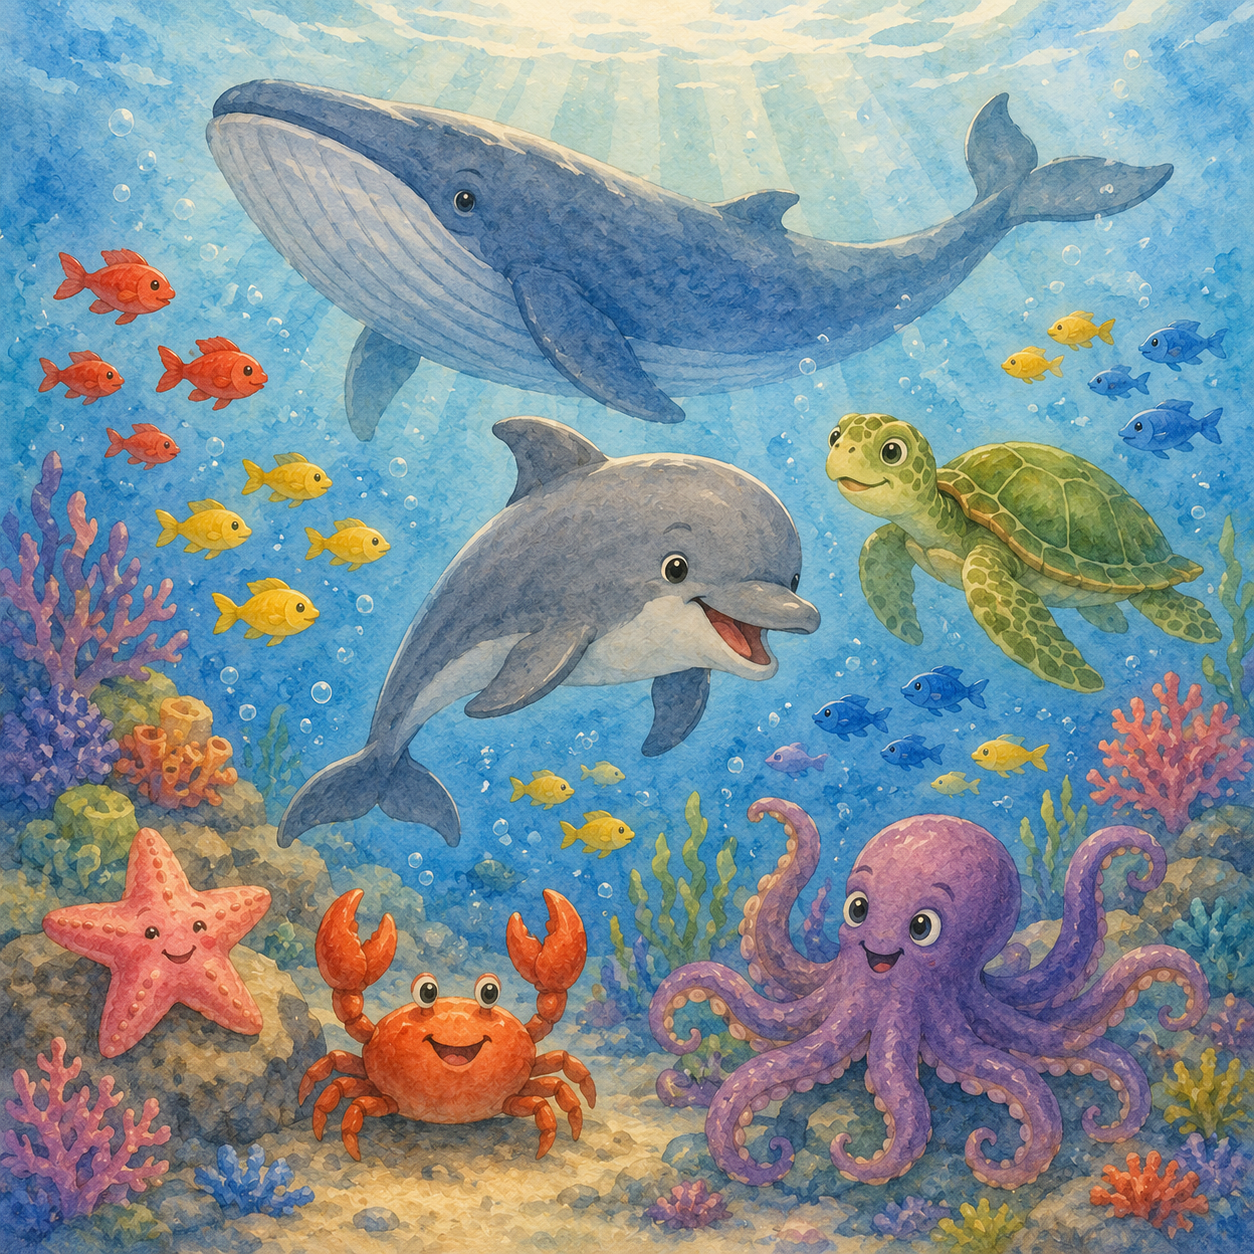
\includegraphics[width=7cm]{img/mer.png}
\end{wrapfigure}

La tortue de mer avance toujours lentement. Sa grosse carapace la
protège bien. Elle pond ses œufs sur la plage. Les bébés courent vite
vers l'eau.

Le crabe marche sur le côté avec ses huit pattes. Attention à ses deux
belles pinces ! Il habite près des rochers.

L'étoile de mer a cinq beaux bras. Elle se promène lentement sur les
rochers. On la trouve rose, orange ou rouge.

Le dauphin, lui, est très intelligent. Il nage vite et saute hors de
l'eau. Il adore jouer avec les bateaux. Pour parler, il fait des petits
sons rigolos.

Connais-tu la baleine ? C'est le plus grand animal du monde ! Elle vit
dans les mers froides. Pour manger, elle avale des milliers de minuscules
crevettes appelées krills.

La pieuvre, elle, a un super pouvoir. Elle change de couleur en un clin
d'œil. Ses huit bras lui servent à tout attraper.

Tous ces animaux vivent ensemble dans la mer. Lequel est ton préféré ?

\begin{center}\rule{0.5\linewidth}{0.5pt}\end{center}

\subsubsection{Questions de
compréhension}\label{questions-de-compruxe9hension}

\begin{enumerate}
\def\labelenumi{\arabic{enumi}.}
\tightlist
\item
  Quel est le plus grand animal du monde ?
\item
  Combien de pattes a le crabe ?
\item
  Comment la pieuvre se cache-t-elle ?
\end{enumerate}

\begin{center}\rule{0.5\linewidth}{0.5pt}\end{center}

\subsubsection{Mon suivi de lecture}\label{mon-suivi-de-lecture}

\begin{center}
\begin{tabularx}{0.75\textwidth}{|X|X|}
\hline
\textbf{Date} & \textbf{Temps} \\
\hline
& \\
\hline
& \\
\hline
& \\
\hline
& \\
\hline
& \\
\hline
\end{tabularx}
\end{center}

\newpage

\section{Je fais du vélo}\label{je-fais-du-vuxe9lo}

\begin{wrapfigure}{r}{7cm}
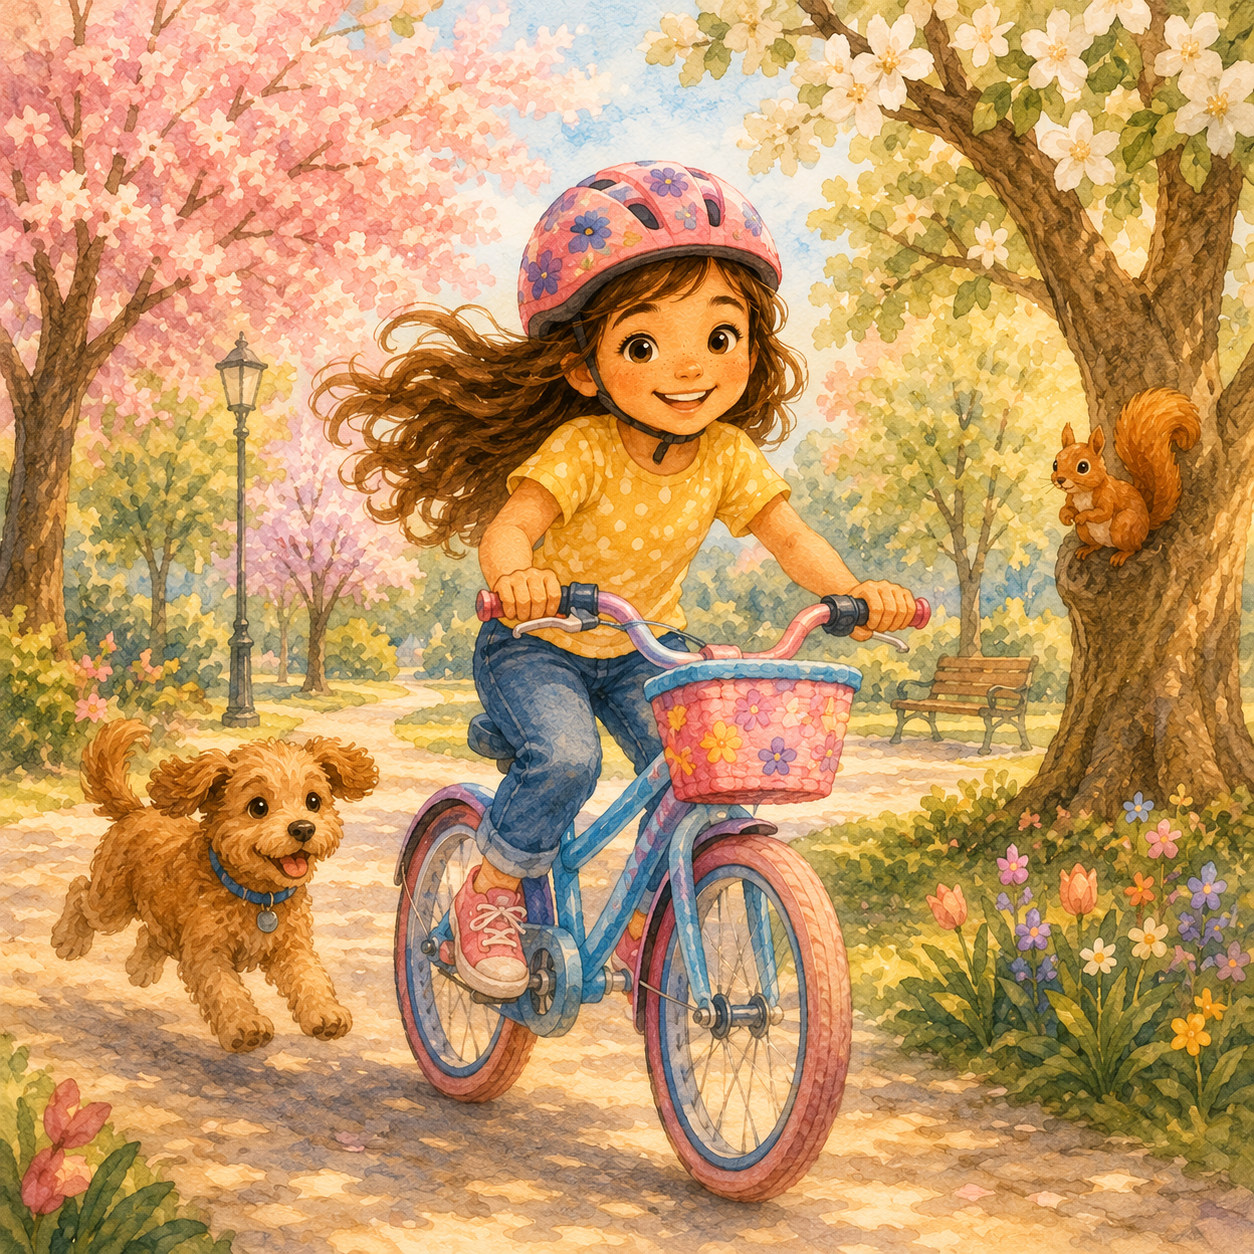
\includegraphics[width=7cm]{img/velo.png}
\end{wrapfigure}

Mon sport préféré, c'est le vélo. J'ai un beau vélo bleu et rose. Il a
deux roues et une petite sonnette. Elle fait « dring dring » quand
j'appuie.

Aujourd'hui, maman et moi allons au parc. Avant de partir, je mets mon
casque. Il protège bien ma tête.

Je monte sur mon vélo. Mes pieds se posent sur les pédales. Je pousse
fort et le vélo avance.

Au début, j'ai un peu peur. Maman tient le vélo par derrière. Puis elle
me lâche doucement. Je roule toute seule ! Je suis très fière de moi.

Le vent souffle dans mes cheveux. C'est super agréable. Je passe devant
les arbres en fleurs. Je vois même un petit chien et un écureuil.

Tout à coup, le chemin descend. Mon vélo va beaucoup trop vite ! Je
serre vite les freins. Il ralentit doucement.

Arrivée au parc, je m'arrête. Je bois un peu d'eau. Maman me regarde
avec un grand sourire. Elle est fière de moi. Moi aussi, je suis très
contente.

Le vélo, c'est vraiment génial !

\newpage

\begin{center}\rule{0.5\linewidth}{0.5pt}\end{center}

\subsubsection{Questions de
compréhension}\label{questions-de-compruxe9hension-1}

\begin{enumerate}
\def\labelenumi{\arabic{enumi}.}
\tightlist
\item
  De quelle couleur est le vélo ?
\item
  Que met la narratrice sur sa tête avant de partir ?
\item
  Pourquoi serre-t-elle les freins ?
\end{enumerate}

\begin{center}\rule{0.5\linewidth}{0.5pt}\end{center}

\subsubsection{Mon suivi de lecture}\label{mon-suivi-de-lecture-1}

\begin{center}
\begin{tabularx}{0.75\textwidth}{|X|X|}
\hline
\textbf{Date} & \textbf{Temps} \\
\hline
& \\
\hline
& \\
\hline
& \\
\hline
& \\
\hline
& \\
\hline
\end{tabularx}
\end{center}

\newpage

\section{Ma copine Sara}\label{ma-copine-sara}

\begin{wrapfigure}{r}{7cm}
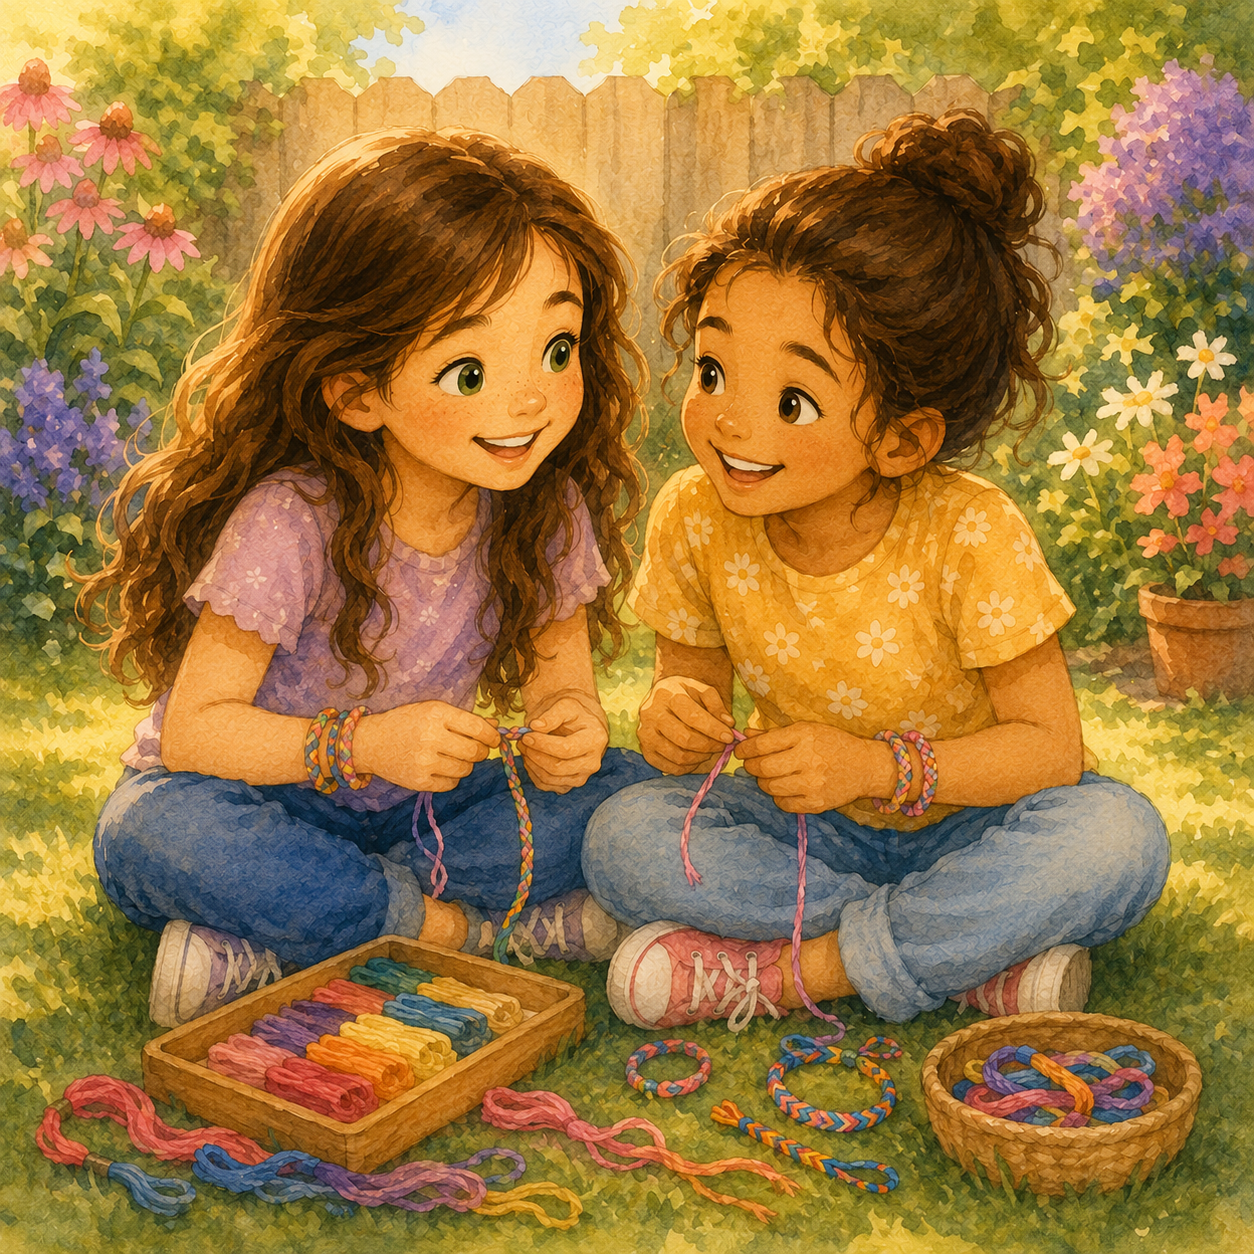
\includegraphics[width=7cm]{img/amie.png}
\end{wrapfigure}

Ma meilleure amie s'appelle Sara. Elle a huit ans, comme moi. Nous
sommes dans la même classe à l'école.

Elle a de longs cheveux bruns et des yeux verts. Elle rit tout le temps.
Son rire est très joyeux.

À la récré, on est toujours ensemble. On adore la corde à sauter et le
dessin. Parfois, on chante des chansons rigolotes. Sara invente même des
jeux que personne ne connaît.

Elle habite tout près de chez moi. Le mercredi, je vais chez elle pour
jouer. On fait des bracelets brésiliens. On joue dans le jardin. Sa
maman nous prépare un goûter délicieux.

Quand je suis triste, Sara me console toujours. Elle me dit des mots
tout doux. Et quand elle est triste, moi je fais pareil. C'est ça, une
vraie amie.

Pour mon anniversaire, elle me fait toujours un beau dessin. Sur le
dessin, on rit ensemble toutes les deux.

Parfois, ça nous arrive de nous disputer. C'est souvent pour pas
grand-chose. On boude un petit moment. Mais on fait vite la paix.

Sara, c'est ma meilleure amie. Je l'aime très fort.

\newpage

\begin{center}\rule{0.5\linewidth}{0.5pt}\end{center}

\subsubsection{Questions de
compréhension}\label{questions-de-compruxe9hension-2}

\begin{enumerate}
\def\labelenumi{\arabic{enumi}.}
\tightlist
\item
  Quel âge a Sara ?
\item
  Que font les deux amies à la récré ?
\item
  Que fait Sara quand la narratrice est triste ?
\end{enumerate}

\begin{center}\rule{0.5\linewidth}{0.5pt}\end{center}

\subsubsection{Mon suivi de lecture}\label{mon-suivi-de-lecture-2}

\begin{center}
\begin{tabularx}{0.75\textwidth}{|X|X|}
\hline
\textbf{Date} & \textbf{Temps} \\
\hline
& \\
\hline
& \\
\hline
& \\
\hline
& \\
\hline
& \\
\hline
\end{tabularx}
\end{center}

\newpage

\section{Ma cabane secrète}\label{ma-cabane-secruxe8te}

\begin{wrapfigure}{r}{7cm}
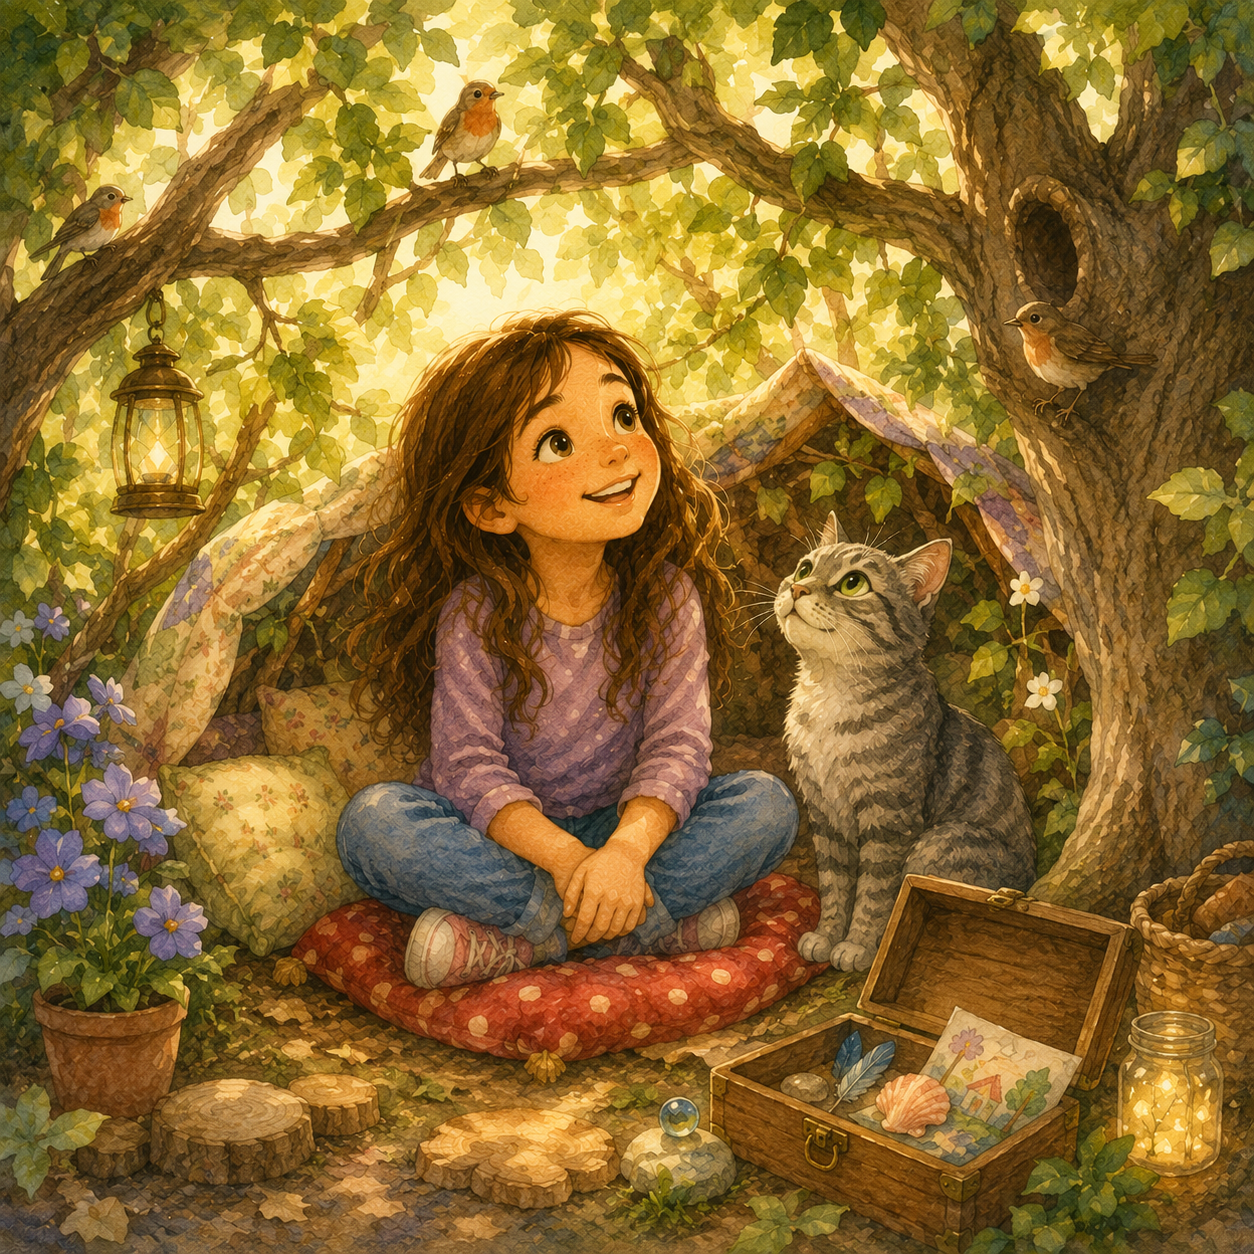
\includegraphics[width=7cm]{img/cabane.png}
\end{wrapfigure}

Au fond de mon jardin, il y a un grand arbre. Sous ses branches, on ne
voit rien depuis dehors. C'est mon endroit préféré au monde.

C'est ma cabane secrète. Personne ne la connaît, pas même mon petit
frère.

Pour entrer, j'écarte deux branches comme un rideau. À l'intérieur, tout
est vert et doux. Le sol est couvert de feuilles mortes. Au-dessus, je
vois le ciel entre les branches.

Sur le sol, il y a un coussin rouge. Il a de petits pois blancs. À côté,
il y a une petite boîte en bois. Dedans, je cache tous mes trésors.

Dans ma boîte, j'ai un caillou brillant. J'ai aussi une plume bleue et
un coquillage. Et un petit dessin de moi.

Quand je suis dans ma cabane, je rêve très fort. Je deviens une
princesse ou une grande exploratrice. Parfois, je suis même une fée
magique.

Mon chat me trouve souvent. Il vient s'asseoir tout près de moi. Sans
faire de bruit, on regarde les oiseaux ensemble.

J'aime beaucoup ma cabane secrète. Dès que je suis triste ou fâchée, je
viens ici. Et tout de suite, je me sens beaucoup mieux.

Cette cabane, c'est mon petit royaume à moi.

\begin{center}\rule{0.5\linewidth}{0.5pt}\end{center}

\subsubsection{Questions de
compréhension}\label{questions-de-compruxe9hension-3}

\begin{enumerate}
\def\labelenumi{\arabic{enumi}.}
\tightlist
\item
  Où est la cabane secrète ?
\item
  Qu'est-ce qu'il y a dans la petite boîte ?
\item
  Pourquoi la narratrice va-t-elle dans sa cabane ?
\end{enumerate}

\begin{center}\rule{0.5\linewidth}{0.5pt}\end{center}

\subsubsection{Mon suivi de lecture}\label{mon-suivi-de-lecture-3}

\begin{center}
\begin{tabularx}{0.75\textwidth}{|X|X|}
\hline
\textbf{Date} & \textbf{Temps} \\
\hline
& \\
\hline
& \\
\hline
& \\
\hline
& \\
\hline
& \\
\hline
\end{tabularx}
\end{center}

\newpage

\sectiondivider{2}{Niveau 1}

\subsubsection{On progresse !}\label{on-progresse}

Les textes de cette section sont un peu plus longs (environ \textbf{270
mots}). Les phrases restent courtes, le vocabulaire reste simple, et
tout est presque toujours au \textbf{présent}.

\subsubsection{Combien de temps pour lire un texte
?}\label{combien-de-temps-pour-lire-un-texte-1}

{\def\LTcaptype{none} % do not increment counter
\begin{longtable}[]{@{}lll@{}}
\toprule\noalign{}
Niveau de référence & Vitesse & Temps pour \textasciitilde270 mots \\
\midrule\noalign{}
\endhead
\bottomrule\noalign{}
\endlastfoot
Fin de CP & 50 mots/min & \textasciitilde5 min 25 s \\
Fin de CE1 & 90 mots/min & \textbf{\textasciitilde{} 3 min} \\
Fin de CE2 & 110 mots/min & \textasciitilde2 min 30 s \\
\end{longtable}
}

\newpage

\section{Mon chat Filou}\label{mon-chat-filou}

\begin{wrapfigure}{r}{7cm}
  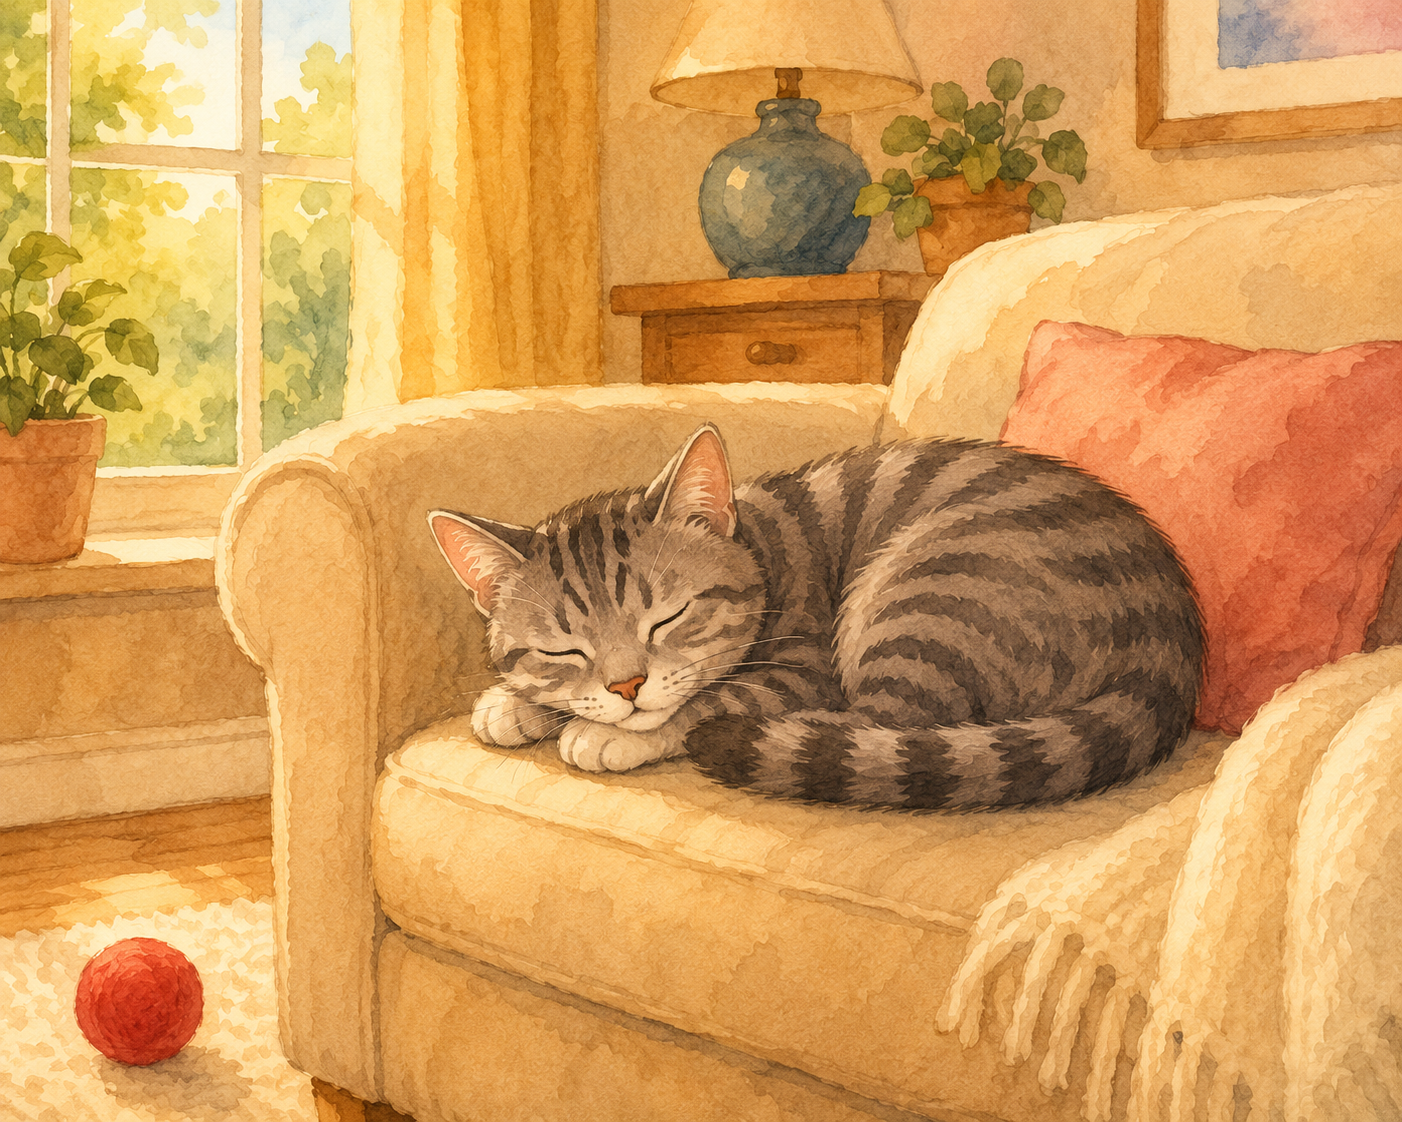
\includegraphics[width=7cm]{img/chat.png}
  \end{wrapfigure}

Filou est mon chat. Il a deux ans. Son pelage est gris avec des rayures
noires. Ses yeux sont verts comme l'herbe.

Filou adore dormir. Le matin, il dort sur mon lit. L'après-midi, il dort
sur le canapé. Le soir, il dort sur le tapis. Maman dit qu'il dort vingt
heures par jour. C'est beaucoup !

Quand il ne dort pas, Filou joue. Il aime sa petite balle rouge. Je la
lance loin et il court derrière. Parfois, il saute très haut pour
l'attraper. Il chasse aussi sa queue, mais il ne l'attrape jamais. Cela
me fait beaucoup rire.

Filou est très gourmand. Il mange ses croquettes deux fois par jour.
Quand j'ouvre le frigo, il arrive tout de suite. Il espère un petit bout
de jambon ou de fromage. Mais maman ne veut pas. Elle dit que ce n'est
pas bon pour lui.

Le soir, Filou monte sur mes genoux. Il ronronne très fort. Cela veut
dire qu'il est heureux. Je caresse son dos tout doux et il ferme les
yeux. C'est mon moment préféré de la journée.

Filou a un petit défaut. Il fait ses griffes sur le canapé. Papa n'est
pas content. Il a acheté un arbre à chat, mais Filou préfère le canapé.
Je crois qu'il fait exprès !

Quand je rentre de l'école, Filou m'attend derrière la porte. Il miaule
pour me dire bonjour. Je suis sûre qu'il m'aime très fort. Et moi aussi,
je l'aime très fort. Filou est mon meilleur ami du monde.

\begin{center}\rule{0.5\linewidth}{0.5pt}\end{center}

\subsubsection{Questions de
compréhension}\label{questions-de-compruxe9hension-4}

\begin{enumerate}
\def\labelenumi{\arabic{enumi}.}
\tightlist
\item
  De quelle couleur est Filou ?
\item
  Combien d'heures par jour dort-il ?
\item
  Pourquoi papa n'est-il pas content ?
\end{enumerate}

\begin{center}\rule{0.5\linewidth}{0.5pt}\end{center}

\subsubsection{Mon suivi de lecture}\label{mon-suivi-de-lecture-4}

\begin{center}
\begin{tabularx}{0.75\textwidth}{|X|X|}
\hline
\textbf{Date} & \textbf{Temps} \\
\hline
& \\
\hline
& \\
\hline
& \\
\hline
& \\
\hline
& \\
\hline
\end{tabularx}
\end{center}

\begin{center}\rule{0.5\linewidth}{0.5pt}\end{center}

\newpage

\section{Je plante des radis}\label{je-plante-des-radis}

\begin{wrapfigure}{r}{7cm}
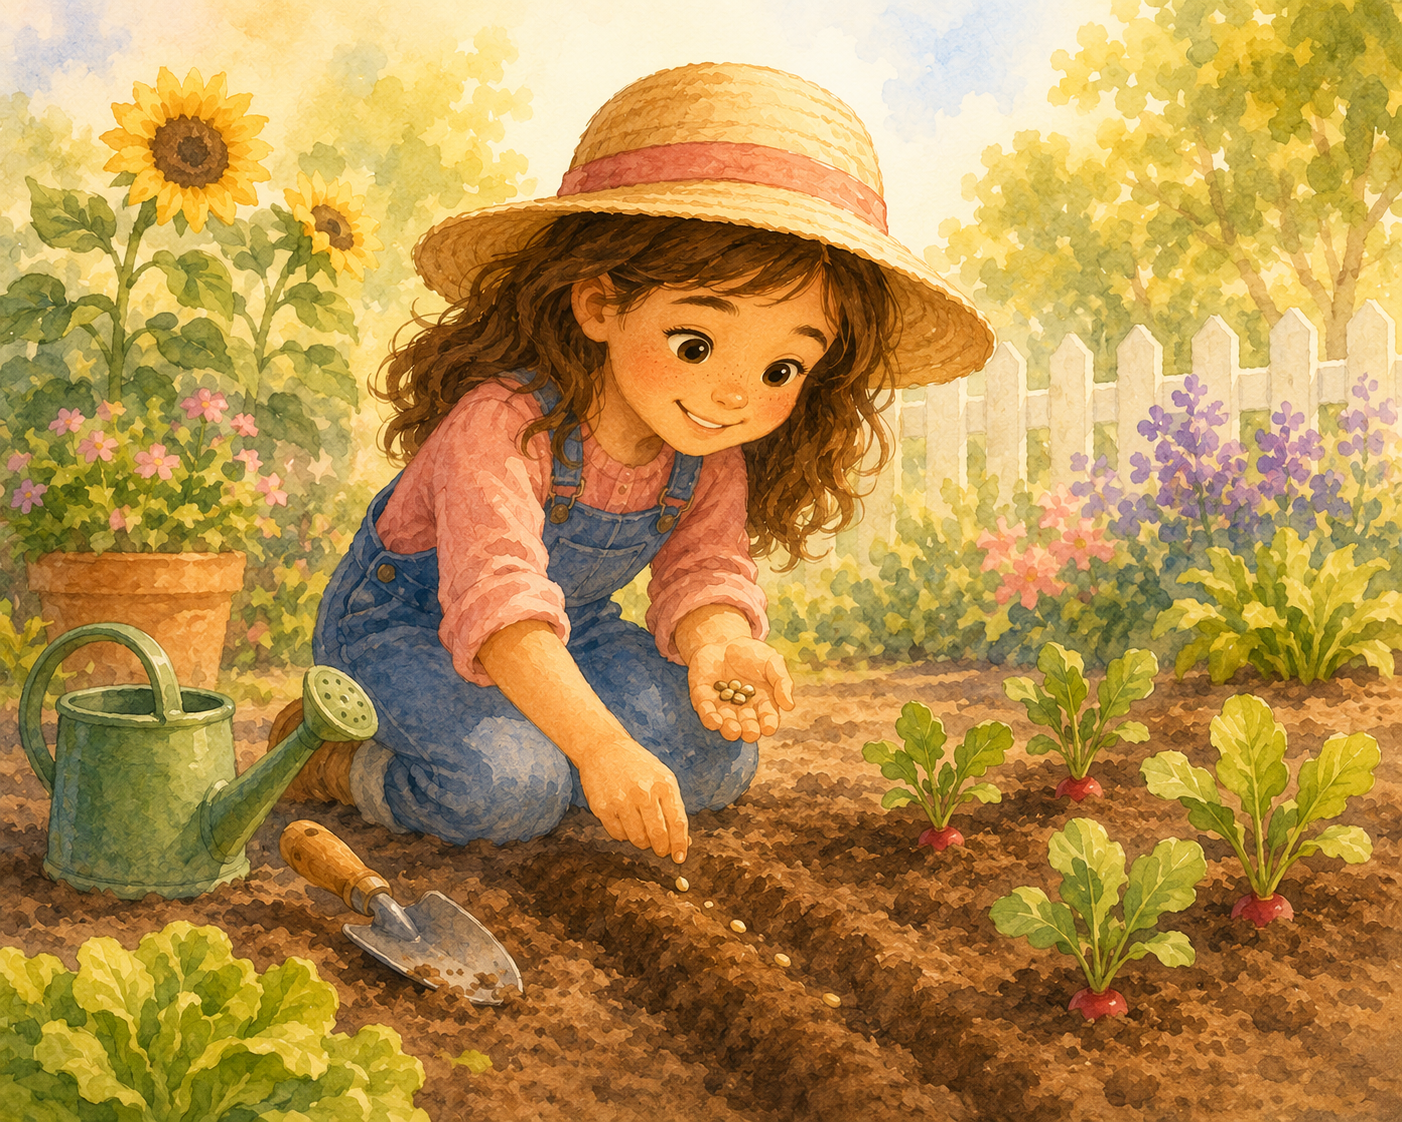
\includegraphics[width=7cm]{img/radis.png}
\end{wrapfigure}

Les radis sont faciles à faire pousser. Tu peux en planter dans un
jardin ou dans un pot sur le balcon. Voici comment faire.

\textbf{Ce qu'il te faut :}

\begin{itemize}
\tightlist
\item
  un sachet de graines de radis
\item
  de la terre
\item
  un petit pot, ou un coin de jardin
\item
  un arrosoir avec de l'eau
\item
  une petite pelle
\end{itemize}

\textbf{Les étapes :}

\begin{enumerate}
\def\labelenumi{\arabic{enumi}.}
\item
  Choisis un endroit au soleil. Les radis aiment la lumière. Sans
  soleil, ils ne poussent pas bien.
\item
  Avec ta pelle, fais un petit trou dans la terre. Le trou doit être peu
  profond. Un seul centimètre suffit.
\item
  Mets deux ou trois graines dans le trou. Recouvre-les avec un peu de
  terre. Tape doucement avec ta main pour bien fermer.
\item
  Arrose avec ton arrosoir. L'eau doit mouiller toute la terre, mais pas
  trop. Sinon, les graines vont pourrir.
\item
  Pendant les jours qui suivent, arrose chaque matin. La terre ne doit
  jamais être sèche.
\end{enumerate}

\textbf{Et après ?}

Après cinq ou six jours, tu verras de petites feuilles vertes sortir de
la terre. Ce sont tes radis qui poussent. Continue à les arroser tous
les jours.

Au bout de trois ou quatre semaines, tes radis seront prêts. Tu pourras
les tirer doucement par les feuilles. Ils auront une jolie couleur rouge
et blanche.

Lave-les bien à l'eau froide. Ensuite, coupe les feuilles et le petit
bout du bas. Tu peux les manger crus, avec un peu de beurre et de sel.
C'est délicieux.

Bravo, tu as fait pousser tes propres radis !

\begin{center}\rule{0.5\linewidth}{0.5pt}\end{center}

\subsubsection{Questions de
compréhension}\label{questions-de-compruxe9hension-5}

\begin{enumerate}
\def\labelenumi{\arabic{enumi}.}
\tightlist
\item
  De quoi as-tu besoin pour planter des radis ?
\item
  Combien de jours faut-il pour voir les premières feuilles ?
\item
  Comment peut-on manger les radis à la fin ?
\end{enumerate}

\begin{center}\rule{0.5\linewidth}{0.5pt}\end{center}

\subsubsection{Mon suivi de lecture}\label{mon-suivi-de-lecture-5}

\begin{center}
\begin{tabularx}{0.75\textwidth}{|X|X|}
\hline
\textbf{Date} & \textbf{Temps} \\
\hline
& \\
\hline
& \\
\hline
& \\
\hline
& \\
\hline
& \\
\hline
\end{tabularx}
\end{center}

\begin{center}\rule{0.5\linewidth}{0.5pt}\end{center}

\newpage

\section{Le premier jour de Mango}\label{le-premier-jour-de-mango}

\begin{wrapfigure}{r}{7cm}
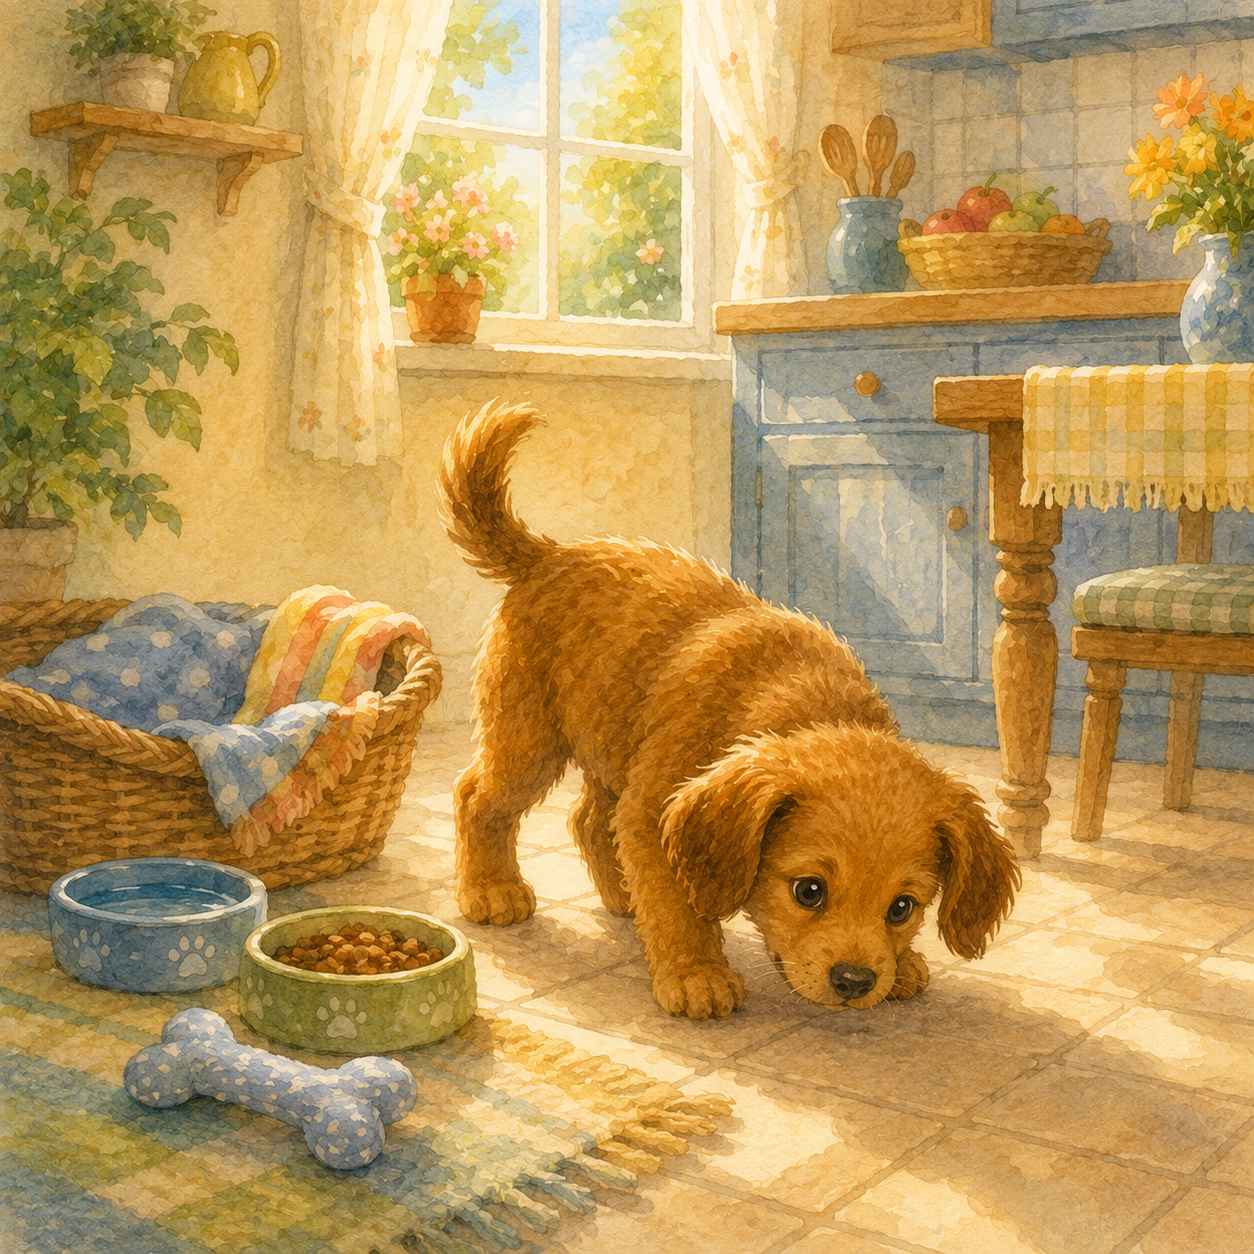
\includegraphics[width=7cm]{img/mango.png}
\end{wrapfigure}

C'est le grand jour. Mango arrive à la maison. Mango est un petit chien
tout brun. Il a deux mois. Il a de grandes oreilles tombantes et une
queue qui ne s'arrête jamais de bouger.

Quand papa pose Mango sur le sol, il tremble un peu. Il regarde partout.
Tout est nouveau pour lui : la maison, les bruits, les odeurs, et nous.
Je m'approche doucement. Je tends ma main. Il sent mes doigts avec
son petit nez froid. Puis il me lèche la main. Je crois qu'il m'aime
déjà !

Maman a tout préparé. Dans un coin de la cuisine, il y a un panier avec
une couverture toute douce. Près du panier, il y a deux gamelles. L'une
pour l'eau, l'autre pour les croquettes. Et aussi un petit jouet en
forme d'os.

Mango va voir son panier. Il monte dedans et se couche en boule. Mais
cinq minutes plus tard, il en sort. Il veut découvrir la maison. Il sent
chaque coin, chaque meuble. Il met même son nez dans mes chaussures !

À midi, il mange ses croquettes pour la première fois. Il les avale
très vite. Ensuite, il boit beaucoup d'eau.

L'après-midi, je joue avec lui. Je lance la petite balle dans le jardin.
Mango court derrière en aboyant. Il est rapide ! Mais il ne me rapporte
pas la balle. Il préfère la mâcher dans son coin.

Le soir, Mango est très fatigué. Il s'endort dans son panier. Je le
regarde dormir. Je me dis que ma vie va changer. Maintenant, j'ai un
meilleur ami à quatre pattes.

\begin{center}\rule{0.5\linewidth}{0.5pt}\end{center}

\subsubsection{Questions de
compréhension}\label{questions-de-compruxe9hension-6}

\begin{enumerate}
\def\labelenumi{\arabic{enumi}.}
\tightlist
\item
  Quel âge a Mango ?
\item
  Qu'a préparé maman pour lui dans la cuisine ?
\item
  Pourquoi Mango ne rapporte-t-il pas la balle ?
\end{enumerate}

\begin{center}\rule{0.5\linewidth}{0.5pt}\end{center}

\subsubsection{Mon suivi de lecture}\label{mon-suivi-de-lecture-6}

\begin{center}
\begin{tabularx}{0.75\textwidth}{|X|X|}
\hline
\textbf{Date} & \textbf{Temps} \\
\hline
& \\
\hline
& \\
\hline
& \\
\hline
& \\
\hline
& \\
\hline
\end{tabularx}
\end{center}

\begin{center}\rule{0.5\linewidth}{0.5pt}\end{center}

\newpage

\section{À la patinoire}\label{uxe0-la-patinoire}

\begin{wrapfigure}{r}{7cm}
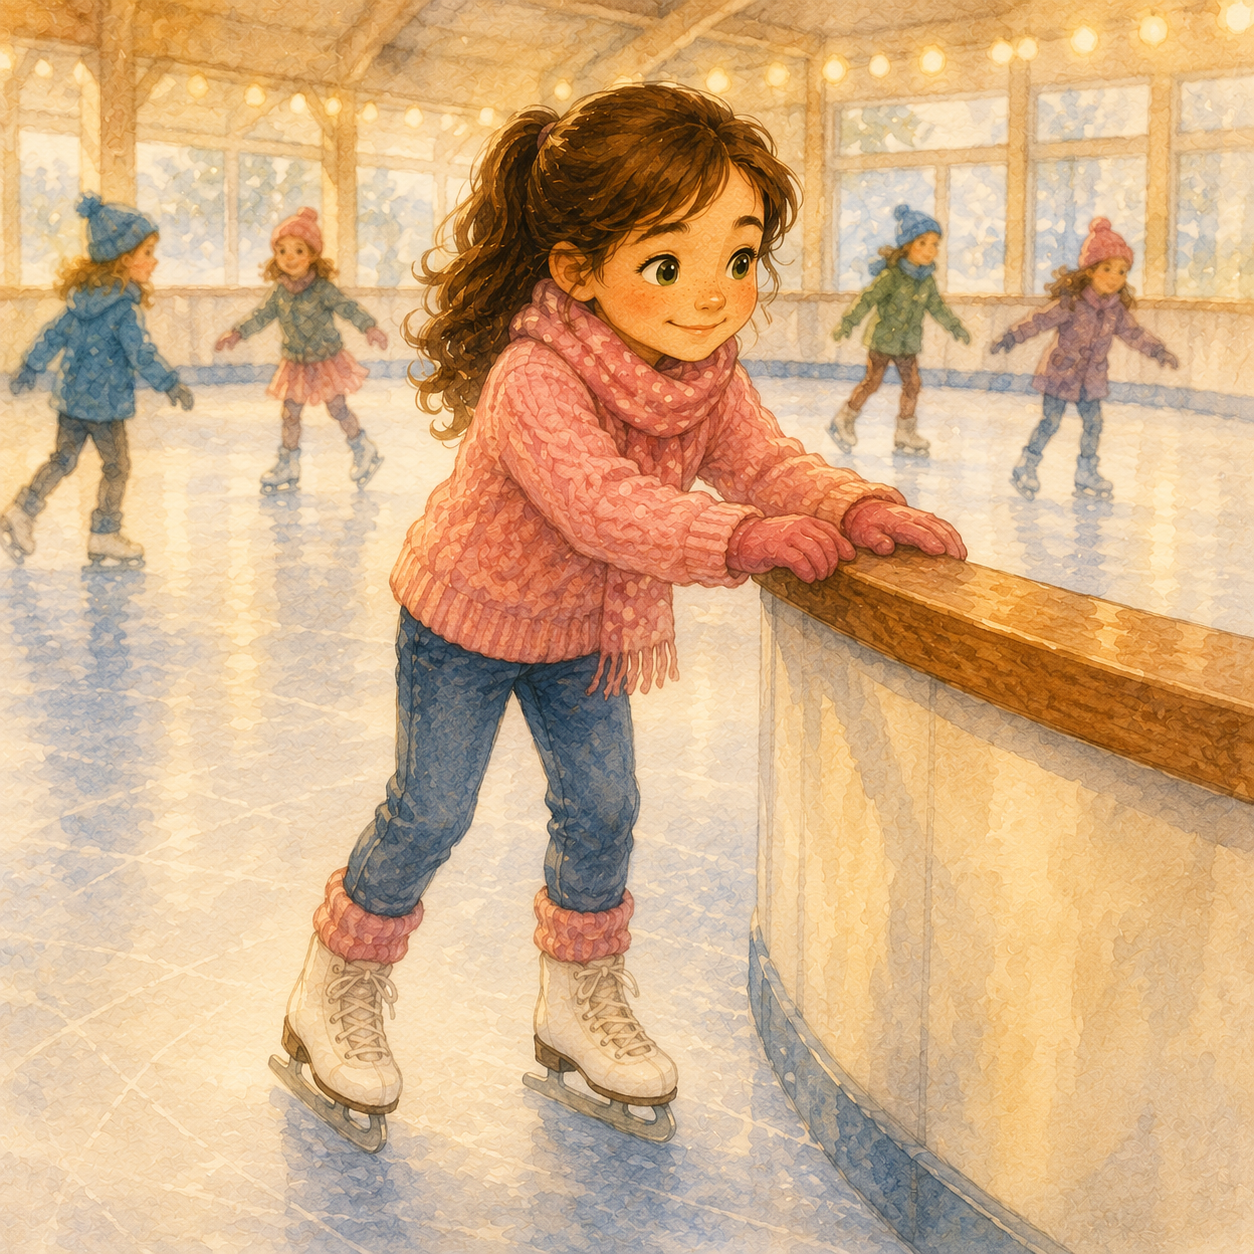
\includegraphics[width=7cm]{img/patinoire.png}
\end{wrapfigure}

C'est samedi matin. Je vais à la patinoire pour la première fois. J'ai
un peu peur. Maman me prend par la main. Elle me dit que tout va bien se
passer.

Devant la patinoire, il y a une longue file. Beaucoup d'enfants
attendent comme moi. Quand c'est mon tour, je donne mes chaussures. La
dame me prête une paire de patins. Ils sont blancs avec des lacets très
longs. Je les mets et papa serre bien les lacets. Mes pieds se sentent
serrés et durs.

Je marche sur les patins. C'est difficile ! On dirait que je vais tomber
à chaque pas. J'arrive enfin devant la glace. Elle brille comme un
miroir. Tout autour, il y a une grande barrière en bois.

Je pose un pied sur la glace. Puis l'autre. Je tiens fort la barrière.
La glace est dure et froide. Je glisse un peu et j'ai très peur. Mais je
ne tombe pas.

Tout à coup, un garçon passe à côté de moi. Il glisse très vite. Il fait
même un petit saut ! Je le regarde, étonnée. Je voudrais bien faire
pareil, mais je ne sais pas.

Maman vient près de moi. Elle me prend les mains. « Plie un peu les
genoux », dit-elle. J'essaie. Je glisse doucement. Je fais quelques pas.
Et puis\ldots{} patatras ! Je tombe sur les fesses. Je ris très fort. Ce
n'est pas si grave.

Je me relève toute seule. J'essaie encore. Cette fois, je glisse plus
loin. Je commence à aimer ça. À la fin de l'heure, je ne veux plus
partir !

\begin{center}\rule{0.5\linewidth}{0.5pt}\end{center}

\subsubsection{Questions de
compréhension}\label{questions-de-compruxe9hension-7}

\begin{enumerate}
\def\labelenumi{\arabic{enumi}.}
\tightlist
\item
  Pourquoi la fille a-t-elle peur au début ?
\item
  Que fait le garçon qui passe à côté d'elle ?
\item
  Comment se sent-elle à la fin de l'heure ?
\end{enumerate}

\begin{center}\rule{0.5\linewidth}{0.5pt}\end{center}

\subsubsection{Mon suivi de lecture}\label{mon-suivi-de-lecture-7}

\begin{center}
\begin{tabularx}{0.75\textwidth}{|X|X|}
\hline
\textbf{Date} & \textbf{Temps} \\
\hline
& \\
\hline
& \\
\hline
& \\
\hline
& \\
\hline
& \\
\hline
\end{tabularx}
\end{center}

\begin{center}\rule{0.5\linewidth}{0.5pt}\end{center}

\newpage

\sectiondivider{3}{Niveau 2}

\subsubsection{Un peu plus riche}\label{un-peu-plus-riche}

Les textes de cette section font environ \textbf{360 mots}. Les phrases
sont un peu plus longues. On y rencontre du \textbf{présent}, de
\textbf{l'imparfait} et du \textbf{passé composé}. Le vocabulaire
devient plus varié.

\subsubsection{Combien de temps pour lire un texte
?}\label{combien-de-temps-pour-lire-un-texte-2}

{\def\LTcaptype{none} % do not increment counter
\begin{longtable}[]{@{}lll@{}}
\toprule\noalign{}
Niveau de référence & Vitesse & Temps pour \textasciitilde360 mots \\
\midrule\noalign{}
\endhead
\bottomrule\noalign{}
\endlastfoot
Fin de CP & 50 mots/min & \textasciitilde7 min 10 s \\
Fin de CE1 & 90 mots/min & \textbf{\textasciitilde{} 4 min} \\
Fin de CE2 & 110 mots/min & \textasciitilde3 min 15 s \\
\end{longtable}
}

\newpage

\section{Les habitants de la forêt}\label{les-habitants-de-la-foruxeat}

\begin{wrapfigure}{r}{7cm}
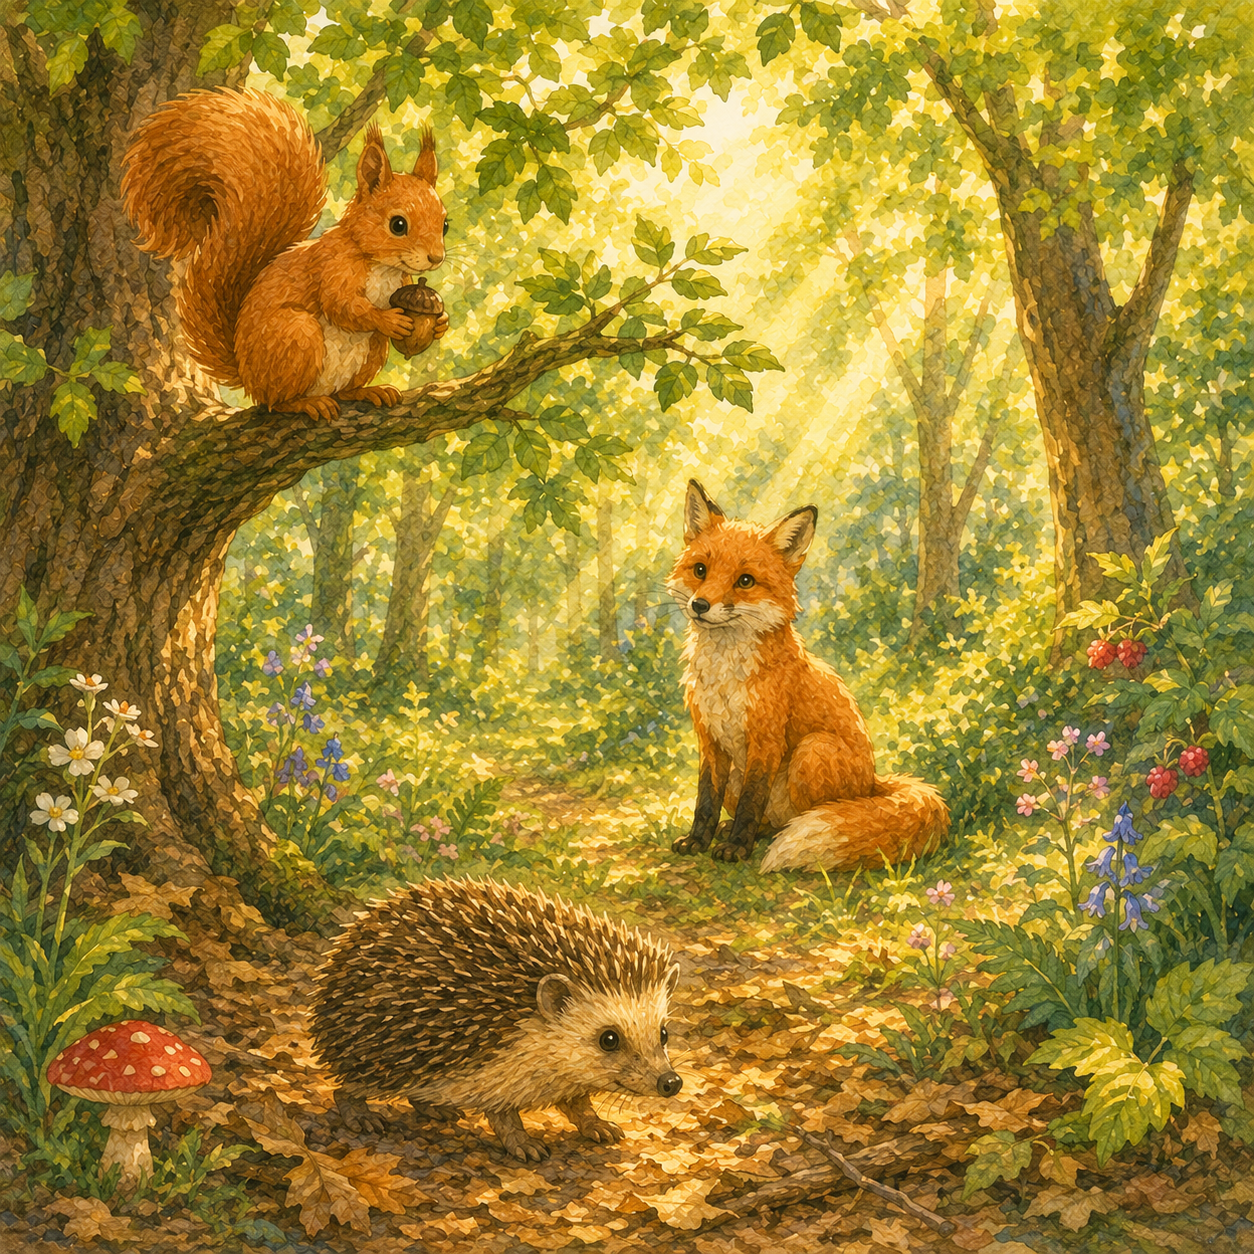
\includegraphics[width=7cm]{img/foret.png}
\end{wrapfigure}

La forêt est pleine de vie. Beaucoup d'animaux y vivent en cachette.
Certains sont faciles à voir. D'autres se cachent très bien. Voici trois
habitants importants de nos forêts.

\textbf{Le hérisson}

Le hérisson est un petit animal couvert de piquants. Il mesure environ
vingt-cinq centimètres. Son dos est plein de piquants durs. Quand il a
peur, il se met en boule. Comme cela, les autres animaux ne peuvent pas
le manger.

Le hérisson dort le jour. La nuit, il cherche à manger. Il aime les vers
de terre, les escargots et les insectes. En hiver, il dort pendant
plusieurs mois. On appelle ce long sommeil l'hibernation.

\textbf{L'écureuil roux}

L'écureuil roux est très rapide. Il vit dans les arbres. Sa queue est
longue et touffue. Elle l'aide à garder l'équilibre quand il saute de
branche en branche.

L'écureuil aime les noisettes, les glands et les graines. En automne, il
fait des réserves. Il cache de la nourriture dans plusieurs endroits
différents. Mais il oublie souvent où il les a mises ! Ces graines
oubliées deviennent parfois de nouveaux arbres.

\textbf{Le renard}

Le renard ressemble un peu à un petit chien. Il a un beau pelage roux et
une queue épaisse. C'est un animal rusé. Il se déplace surtout le soir
et la nuit.

Le renard chasse les petits animaux : souris, lapins, oiseaux. Il mange
aussi des fruits et des œufs. Il vit dans un trou qu'on appelle un
terrier. C'est là qu'il élève ses petits, qui s'appellent les
renardeaux.

\textbf{Et les autres ?}

Bien sûr, beaucoup d'autres animaux vivent dans la forêt. Il y a les
chevreuils, les sangliers, les hiboux, les blaireaux\ldots{} Sans
oublier les milliers d'insectes et les oiseaux. Chaque animal a sa
place. Chacun aide la forêt à rester en bonne santé.

La prochaine fois que tu te promènes dans les bois, ouvre bien les yeux
et les oreilles. Tu verras peut-être un de ces animaux !

\begin{center}\rule{0.5\linewidth}{0.5pt}\end{center}

\subsubsection{Questions de
compréhension}\label{questions-de-compruxe9hension-8}

\begin{enumerate}
\def\labelenumi{\arabic{enumi}.}
\tightlist
\item
  Que fait le hérisson quand il a peur ?
\item
  Comment l'écureuil aide-t-il, sans le savoir, à faire pousser de
  nouveaux arbres ?
\item
  Quand le renard sort-il chasser ?
\end{enumerate}

\begin{center}\rule{0.5\linewidth}{0.5pt}\end{center}

\subsubsection{Mon suivi de lecture}\label{mon-suivi-de-lecture-8}

\begin{center}
\begin{tabularx}{0.75\textwidth}{|X|X|}
\hline
\textbf{Date} & \textbf{Temps} \\
\hline
& \\
\hline
& \\
\hline
& \\
\hline
& \\
\hline
& \\
\hline
\end{tabularx}
\end{center}

\begin{center}\rule{0.5\linewidth}{0.5pt}\end{center}

\newpage

\section{Une journée à Tokyo}\label{une-journuxe9e-uxe0-tokyo}

\begin{wrapfigure}{r}{7cm}
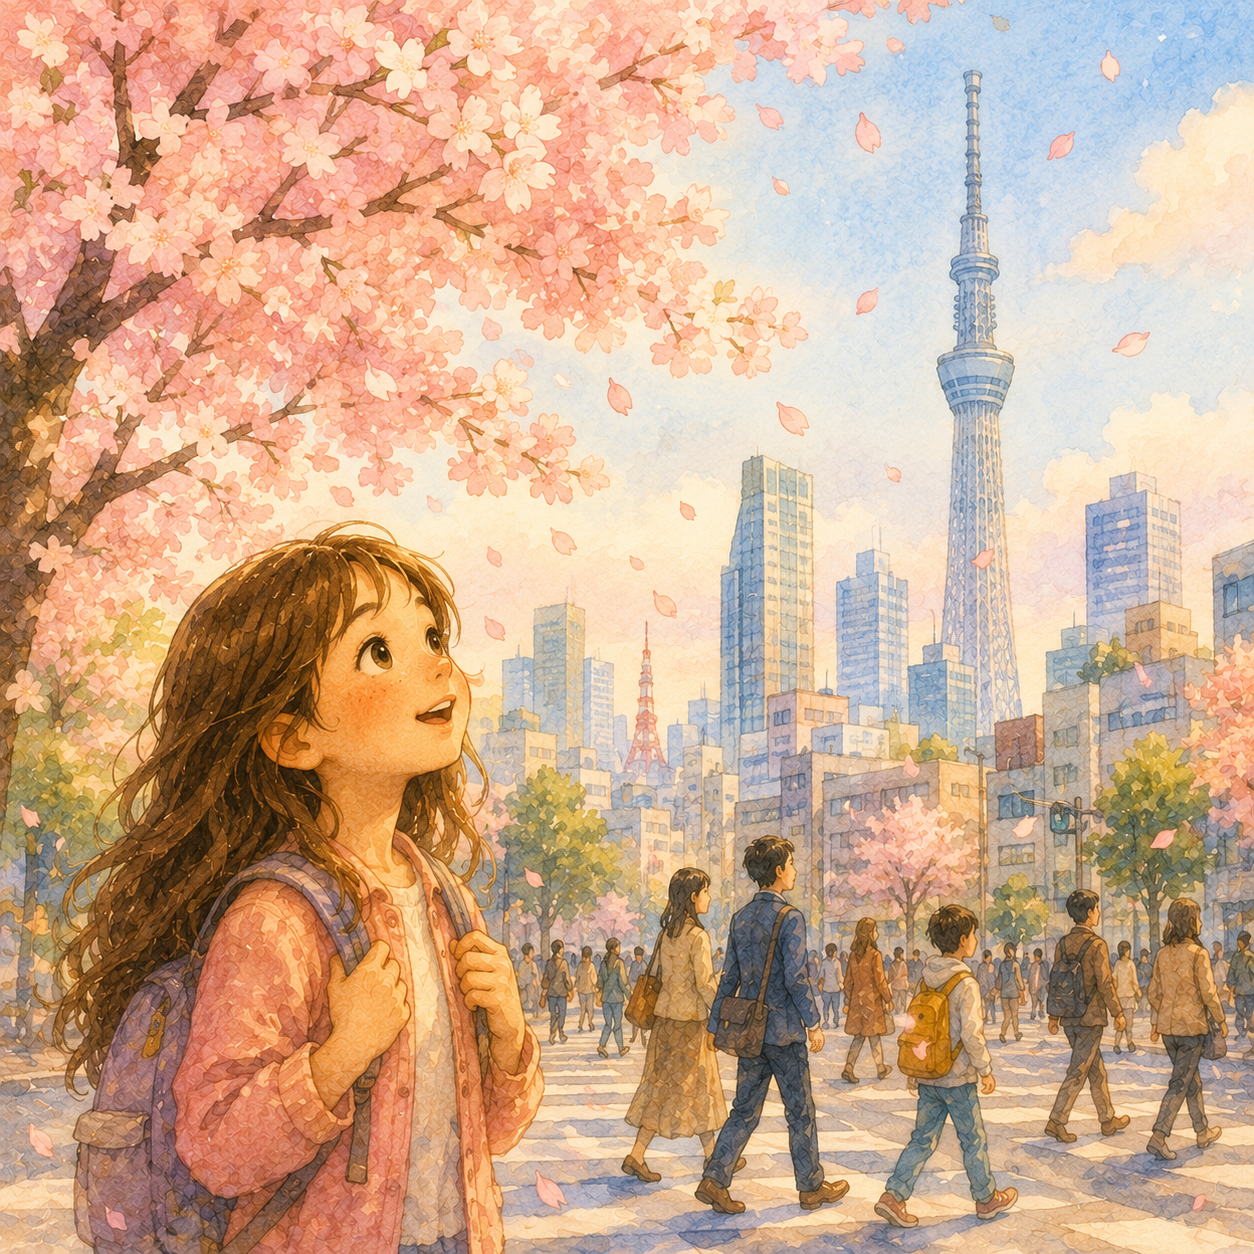
\includegraphics[width=7cm]{img/tokyo.png}
\end{wrapfigure}

Aujourd'hui, je suis à Tokyo, la capitale du Japon. C'est très loin de
la France. Pour venir ici, j'ai pris un grand avion. Le voyage a duré
douze heures !

Ce matin, papa nous a réveillés très tôt. À cause du long voyage, mon
corps croit qu'il fait encore nuit. Mais dehors, le soleil brille déjà.
C'est très bizarre.

Nous sommes sortis de l'hôtel. Tokyo est une ville immense. Il y a des
immeubles très hauts partout. Certains touchent presque les nuages. Dans
les rues, beaucoup de gens marchent vite. Tout le monde a l'air pressé.

Nous avons pris le train. Au Japon, les trains sont propres et toujours
à l'heure. Dans le wagon, personne ne parle fort. Les gens lisent ou
regardent leur téléphone en silence. C'est très calme.

Pour déjeuner, nous avons mangé dans un petit restaurant. J'ai goûté des
sushis. Ce sont de petits morceaux de riz avec du poisson cru posé
dessus. J'avais peur, mais c'était délicieux. Maman m'a appris à manger
avec des baguettes. Au début, je faisais tomber le riz partout !

L'après-midi, nous sommes allés dans un grand jardin. Au milieu de la
ville, il y a un endroit tout vert et tout calme. Des arbres en fleurs
s'appellent des cerisiers. Leurs fleurs sont roses et tombent comme de
la neige. C'est magnifique.

Le soir, nous avons marché dans un quartier qui s'appelle Shibuya. Là,
il y a des lumières partout. Des écrans géants montrent des publicités.
Beaucoup de gens traversent la rue en même temps. J'ai compté plus de
cent personnes en un seul passage !

Avant de rentrer à l'hôtel, nous avons acheté des glaces. La mienne
avait le goût de thé vert. C'était un peu bizarre, mais bon.

Maintenant, je suis très fatiguée. Demain, nous visiterons un grand
temple. Le Japon est un pays merveilleux. Tout est différent de chez
moi. Je suis très contente d'être ici. Je n'oublierai jamais ce voyage.

\begin{center}\rule{0.5\linewidth}{0.5pt}\end{center}

\subsubsection{Questions de
compréhension}\label{questions-de-compruxe9hension-9}

\begin{enumerate}
\def\labelenumi{\arabic{enumi}.}
\tightlist
\item
  Combien de temps a duré le voyage en avion ?
\item
  Qu'est-ce que la narratrice a goûté pour le déjeuner ?
\item
  Pourquoi tout le monde est-il silencieux dans le train ?
\end{enumerate}

\begin{center}\rule{0.5\linewidth}{0.5pt}\end{center}

\subsubsection{Mon suivi de lecture}\label{mon-suivi-de-lecture-9}

\begin{center}
\begin{tabularx}{0.75\textwidth}{|X|X|}
\hline
\textbf{Date} & \textbf{Temps} \\
\hline
& \\
\hline
& \\
\hline
& \\
\hline
& \\
\hline
& \\
\hline
\end{tabularx}
\end{center}

\begin{center}\rule{0.5\linewidth}{0.5pt}\end{center}

\newpage

\section{Comment poussent les
plantes}\label{comment-poussent-les-plantes}

\begin{wrapfigure}{r}{7cm}
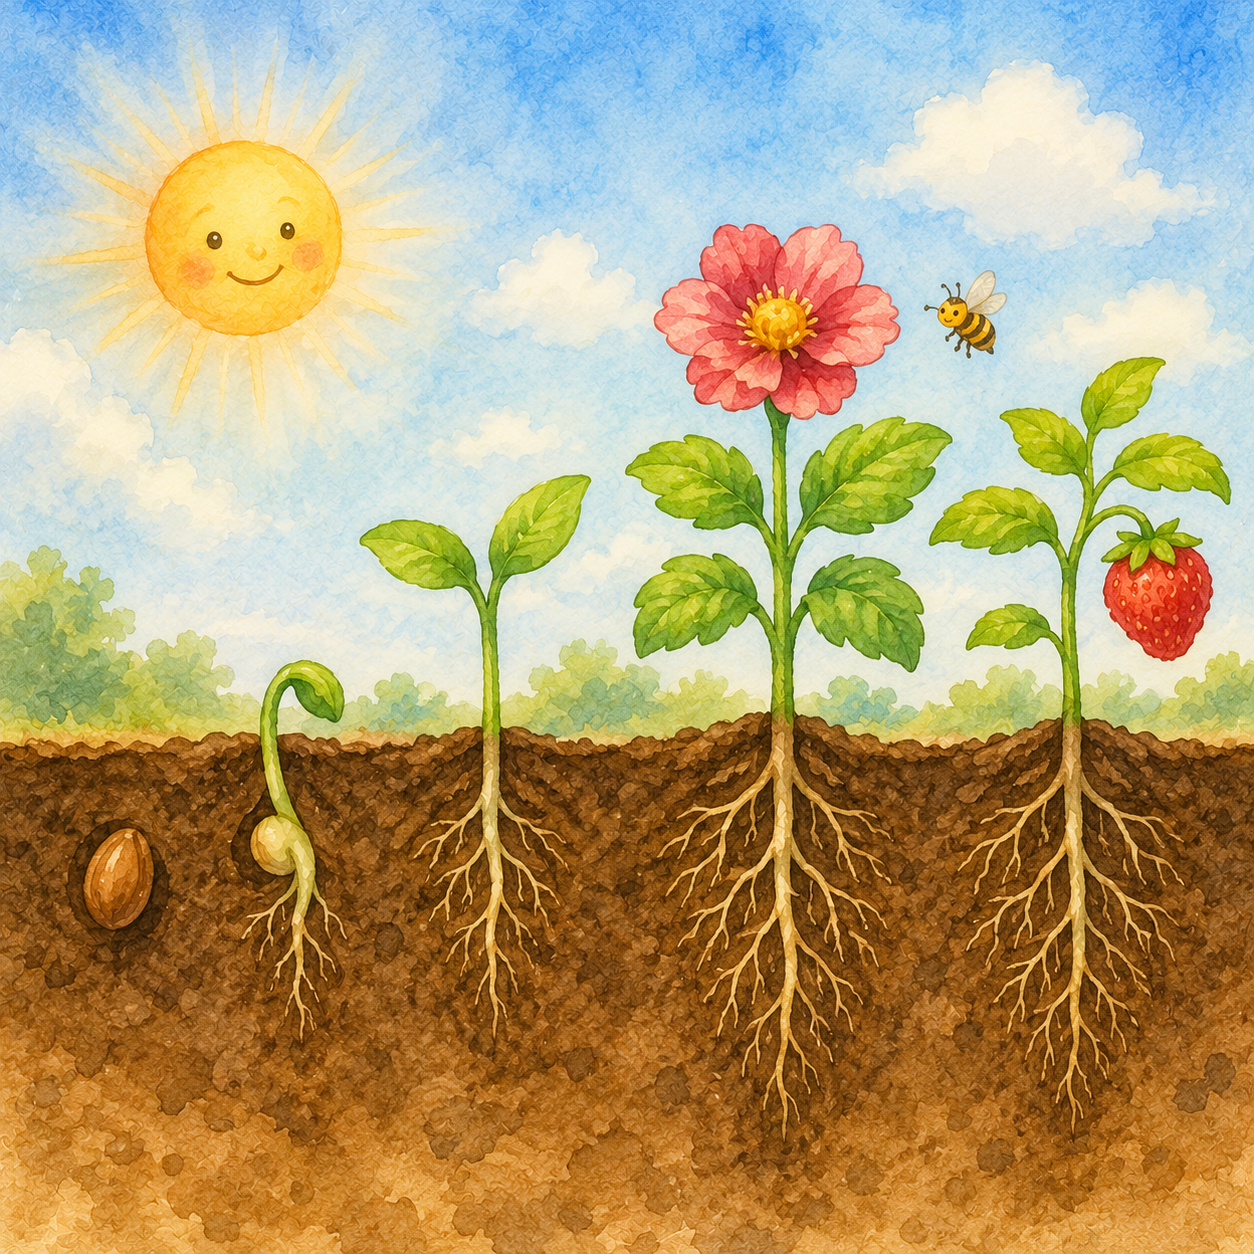
\includegraphics[width=7cm]{img/plantes.png}
\end{wrapfigure}

Toutes les plantes naissent d'une graine. Une graine est très petite,
mais elle est très importante. Elle contient déjà tout ce qu'il faut
pour faire une nouvelle plante.

\textbf{Le début}

Quand on met une graine dans la terre, il ne se passe d'abord rien. Mais
sous la terre, la graine boit l'eau qu'on lui donne. Elle gonfle. Puis,
après quelques jours, une petite racine sort. Elle s'enfonce dans la
terre pour chercher de la nourriture.

Ensuite, une toute petite tige verte sort vers le haut. Elle pousse vers
la lumière du soleil. Bientôt, on voit ses premières feuilles. La plante
est née !

\textbf{Pour pousser, il faut quoi ?}

Une plante a besoin de quatre choses pour bien pousser :

\begin{enumerate}
\def\labelenumi{\arabic{enumi}.}
\tightlist
\item
  \textbf{De l'eau} : elle boit par ses racines.
\item
  \textbf{De la lumière} : ses feuilles aiment le soleil.
\item
  \textbf{De la terre} : elle y trouve sa nourriture.
\item
  \textbf{De l'air} : ses feuilles respirent.
\end{enumerate}

Si l'une de ces choses manque, la plante ne pousse pas bien. Par
exemple, sans eau, elle sèche. Sans soleil, elle devient toute jaune.

\textbf{La fleur et le fruit}

Quand la plante est assez grande, elle fait des fleurs. Les fleurs sont
jolies, mais elles ne servent pas seulement à décorer. Elles servent à
attirer les abeilles et les autres insectes.

Les insectes prennent un peu de poudre jaune sur les fleurs. Cette
poudre s'appelle le pollen. Ils la portent sur d'autres fleurs. Ainsi,
les fleurs peuvent faire des graines.

Plus tard, à la place de la fleur, un fruit apparaît. À l'intérieur du
fruit, il y a de nouvelles graines. Si on plante ces graines, le cycle
peut recommencer.

\textbf{Un cercle qui ne s'arrête jamais}

C'est merveilleux : une seule graine peut donner une grande plante.
Cette plante peut faire des centaines de nouvelles graines. Et chaque
graine peut devenir une nouvelle plante. La nature est très bien faite,
tu ne trouves pas ?

\begin{center}\rule{0.5\linewidth}{0.5pt}\end{center}

\subsubsection{Questions de
compréhension}\label{questions-de-compruxe9hension-10}

\begin{enumerate}
\def\labelenumi{\arabic{enumi}.}
\tightlist
\item
  Quelles sont les quatre choses dont une plante a besoin pour pousser ?
\item
  À quoi servent vraiment les fleurs (en plus d'être jolies) ?
\item
  Que trouve-t-on à l'intérieur d'un fruit ?
\end{enumerate}

\begin{center}\rule{0.5\linewidth}{0.5pt}\end{center}

\subsubsection{Mon suivi de lecture}\label{mon-suivi-de-lecture-10}

\begin{center}
\begin{tabularx}{0.75\textwidth}{|X|X|}
\hline
\textbf{Date} & \textbf{Temps} \\
\hline
& \\
\hline
& \\
\hline
& \\
\hline
& \\
\hline
& \\
\hline
\end{tabularx}
\end{center}

\begin{center}\rule{0.5\linewidth}{0.5pt}\end{center}

\newpage

\section{Le chat des voisins}\label{le-chat-des-voisins}

\begin{wrapfigure}{r}{7cm}
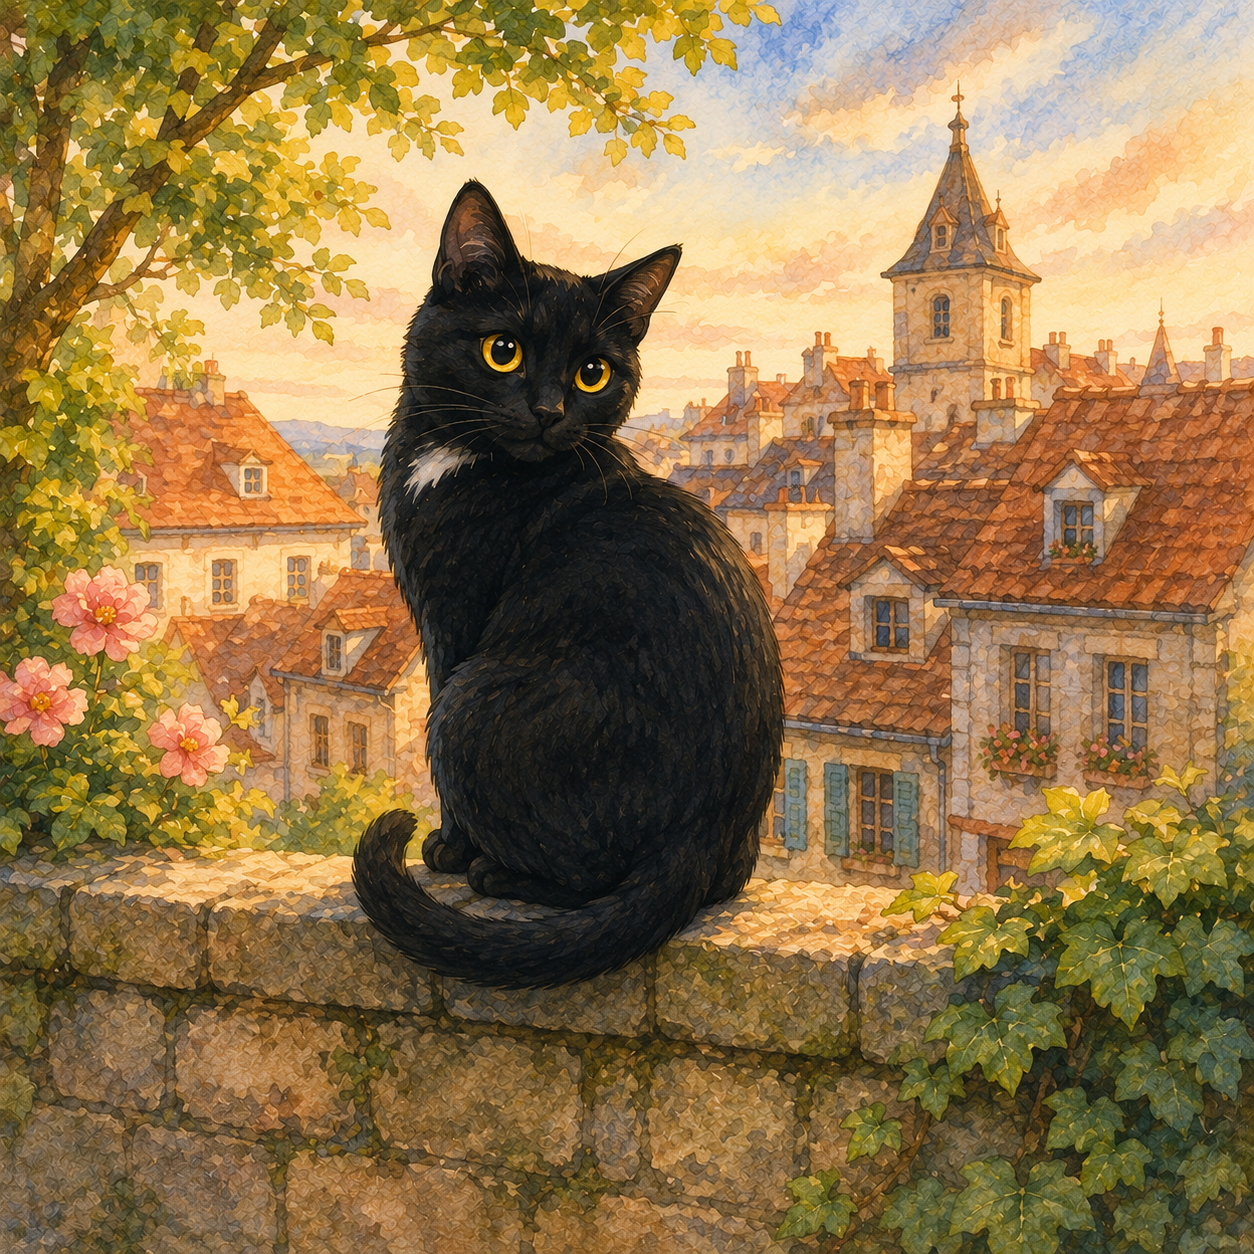
\includegraphics[width=7cm]{img/minuit.png}
\end{wrapfigure}

Depuis trois jours, un chat vient dans notre jardin. Il est tout noir,
sauf une petite tache blanche sous le menton. Personne ne le connaît
dans la rue. D'où vient-il ?

La première fois, je l'ai vu sur le mur. Il me regardait avec ses grands
yeux jaunes. Je n'ai pas bougé. Au bout de quelques minutes, il a sauté
dans l'herbe. Il s'est approché doucement. Je lui ai tendu la main. Il
m'a sentie, puis il est reparti sans bruit.

Le lendemain, il est revenu. Cette fois, il s'est couché au soleil sur
la terrasse. Maman lui a donné un peu de lait. Il a tout bu très vite.
Il avait l'air d'avoir faim. Mais il était propre et son pelage
brillait. Ce n'est sûrement pas un chat perdu.

Le troisième jour, je l'ai suivi en cachette quand il est parti. Il a
marché le long du mur. Il a tourné dans le petit chemin. Il s'est arrêté
devant la maison de madame Lulu, notre voisine. Là, il a miaulé. La
porte s'est ouverte. Et le chat est entré tout droit chez elle !

Alors j'ai compris. Ce chat habite chez madame Lulu. Il s'appelle
Minuit. Madame Lulu me l'a expliqué le soir. Elle a beaucoup ri quand je
lui ai raconté son secret. « Oh, Minuit aime visiter le quartier »,
m'a-t-elle dit. « Il a beaucoup d'amis dans toutes les maisons. Tu n'es
pas la seule à le nourrir ! »

C'est vrai : madame Cohen, au numéro huit, lui donne du poisson.
Monsieur Pierre, en face, lui ouvre sa cuisine quand il pleut. Et le
boulanger lui garde un petit bout de poulet le midi.

Minuit a au moins six maisons et beaucoup de familles. Il est libre
comme l'air. Maintenant, quand je le vois, je lui dis bonjour. Il n'est
pas vraiment mon chat. Mais c'est un peu mon ami quand même. Et c'est
déjà très bien.

\begin{center}\rule{0.5\linewidth}{0.5pt}\end{center}

\subsubsection{Questions de
compréhension}\label{questions-de-compruxe9hension-11}

\begin{enumerate}
\def\labelenumi{\arabic{enumi}.}
\tightlist
\item
  Comment est le chat noir ? (donne deux détails)
\item
  Chez qui habite vraiment Minuit ?
\item
  Pourquoi dit-on que Minuit a « six maisons » ?
\end{enumerate}

\begin{center}\rule{0.5\linewidth}{0.5pt}\end{center}

\subsubsection{Mon suivi de lecture}\label{mon-suivi-de-lecture-11}

\begin{center}
\begin{tabularx}{0.75\textwidth}{|X|X|}
\hline
\textbf{Date} & \textbf{Temps} \\
\hline
& \\
\hline
& \\
\hline
& \\
\hline
& \\
\hline
& \\
\hline
\end{tabularx}
\end{center}

\begin{center}\rule{0.5\linewidth}{0.5pt}\end{center}

\newpage

\sectiondivider{4}{Niveau 3}

\subsubsection{Niveau CE1 complet}\label{niveau-ce1-complet}

Les textes de cette section font environ \textbf{450 mots}. C'est le
niveau attendu en fin de CE1. Le vocabulaire est plus riche, les phrases
peuvent aller jusqu'à 18 mots, et tu rencontreras toutes les
conjugaisons courantes (présent, imparfait, passé composé, futur).

\subsubsection{Combien de temps pour lire un texte
?}\label{combien-de-temps-pour-lire-un-texte-3}

{\def\LTcaptype{none} % do not increment counter
\begin{longtable}[]{@{}lll@{}}
\toprule\noalign{}
Niveau de référence & Vitesse & Temps pour \textasciitilde450 mots \\
\midrule\noalign{}
\endhead
\bottomrule\noalign{}
\endlastfoot
Fin de CP & 50 mots/min & \textasciitilde9 min \\
Fin de CE1 & 90 mots/min & \textbf{\textasciitilde{} 5 min} \\
Fin de CE2 & 110 mots/min & \textasciitilde4 min 05 s \\
\end{longtable}
}

\newpage

\section{Le spectacle sur glace}\label{le-spectacle-sur-glace}

\begin{wrapfigure}{r}{7cm}
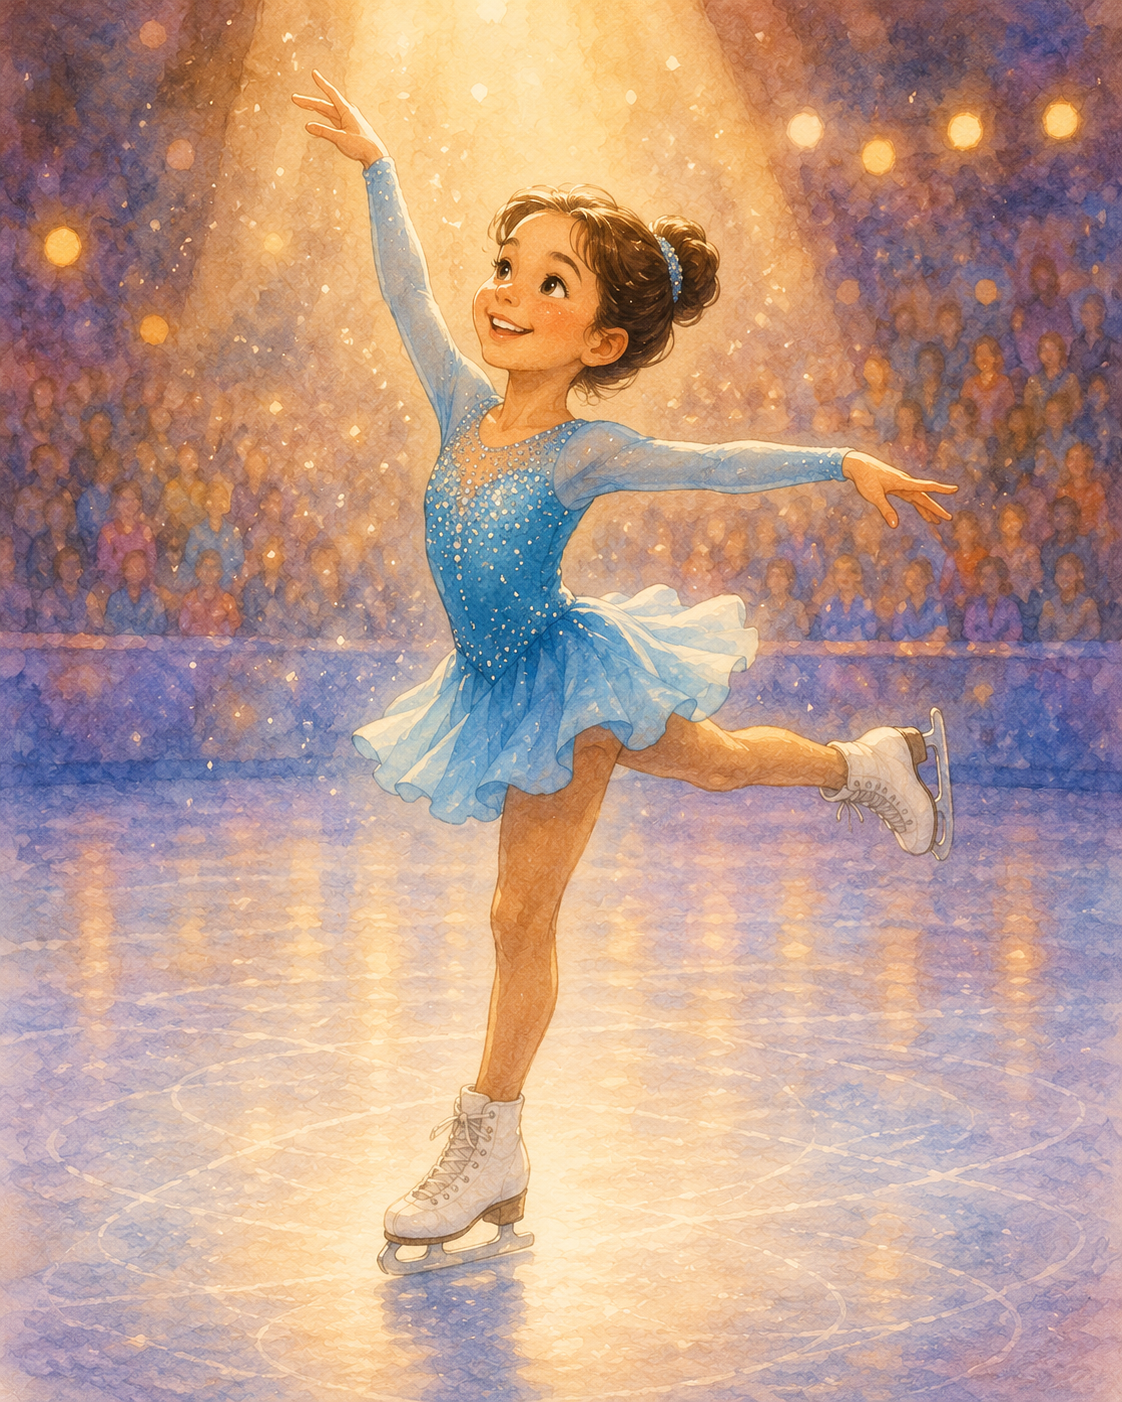
\includegraphics[width=7cm]{img/spectacle.png}
\end{wrapfigure}

Ce soir, c'est le grand jour. Je vais danser sur la glace pour la
première fois devant les gens. Depuis six mois, je m'entraîne avec mon
professeur, madame Léa. Elle dit que je suis prête. Mais moi, je ne suis
pas si sûre.

Dans les vestiaires, beaucoup d'enfants se préparent. Certains rient et
parlent fort. D'autres restent silencieux comme moi. J'ai mis ma jolie
robe bleue. Maman m'a coiffée avec un chignon. Elle m'a aussi mis un peu
de paillettes sur les joues. Je me regarde dans le miroir. Je trouve que
je ressemble à une vraie patineuse.

Madame Léa arrive. Elle nous rassemble en cercle. « Vous êtes
magnifiques », nous dit-elle. « Souriez et amusez-vous. C'est tout ce
que je vous demande. » Mais mon ventre fait des nœuds. Je n'arrive pas à
sourire.

L'heure du spectacle approche. Nous attendons à l'entrée de la
patinoire. La salle est pleine. Il y a beaucoup de papas, de mamans, de
frères et de sœurs. Maman est quelque part dans le public. Je ne la vois
pas.

La musique commence. Mon groupe entre sur la glace. Je suis la
troisième. Quand mon tour arrive, mes jambes tremblent un peu. Je pose
un patin sur la glace, puis l'autre. La lumière est très forte. Tout le
monde me regarde.

Je commence à patiner. Au début, je pense à toutes les choses qu'on a
apprises : les genoux pliés, le dos droit, le sourire. Mais peu à peu,
j'oublie le public. Je suis dans la musique. Mes pieds glissent tout
seuls. Je tourne sur moi-même comme une toupie. Je fais ma figure
préférée : un grand cercle avec un pied en l'air.

Une fois, je glisse un peu trop et je manque de tomber. Mais je tiens
bon. Je continue à sourire, comme madame Léa nous l'a appris. Le public
ne voit rien.

À la fin de la musique, je m'arrête au milieu de la glace. Je lève les
bras vers le haut. Tout le monde applaudit très fort. J'entends même
quelqu'un qui crie « Bravo ! » C'est peut-être papa. Mon cœur bat très
vite, mais je suis très fière.

Quand je sors de la glace, madame Léa me serre dans ses bras. « Tu as
été parfaite », me dit-elle. Maman court vers moi avec un grand bouquet
de fleurs. Elle pleure un peu. Mais c'est de joie.

Je ne sais pas si je serai une grande patineuse plus tard. Mais ce soir,
je suis la patineuse la plus heureuse du monde. Et ça, je ne l'oublierai
jamais.

\begin{center}\rule{0.5\linewidth}{0.5pt}\end{center}

\subsubsection{Questions de
compréhension}\label{questions-de-compruxe9hension-12}

\begin{enumerate}
\def\labelenumi{\arabic{enumi}.}
\tightlist
\item
  Depuis combien de temps la fille s'entraîne-t-elle ?
\item
  Que se passe-t-il pendant son numéro (quand elle glisse trop) ?
\item
  Pourquoi maman pleure-t-elle à la fin ?
\end{enumerate}

\begin{center}\rule{0.5\linewidth}{0.5pt}\end{center}

\subsubsection{Mon suivi de lecture}\label{mon-suivi-de-lecture-12}

\begin{center}
\begin{tabularx}{0.75\textwidth}{|X|X|}
\hline
\textbf{Date} & \textbf{Temps} \\
\hline
& \\
\hline
& \\
\hline
& \\
\hline
& \\
\hline
& \\
\hline
\end{tabularx}
\end{center}

\begin{center}\rule{0.5\linewidth}{0.5pt}\end{center}

\newpage

\section{Médor, le chien qui voit pour
Léon}\label{muxe9dor-le-chien-qui-voit-pour-luxe9on}

\begin{wrapfigure}{r}{7cm}
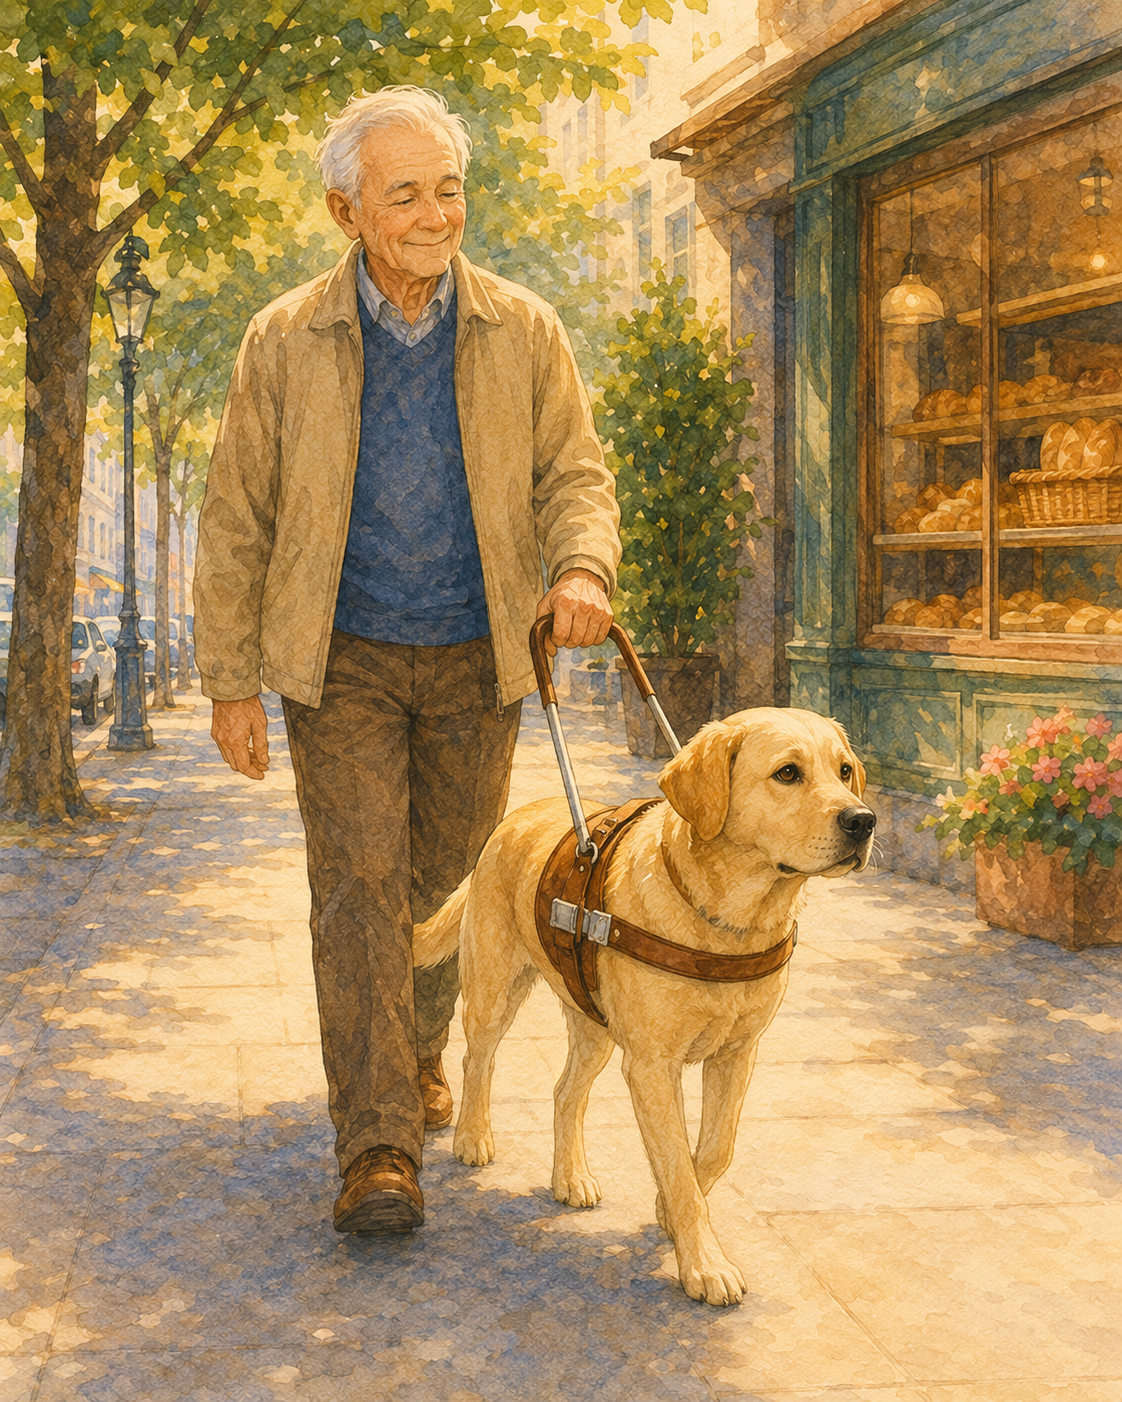
\includegraphics[width=7cm]{img/medor.png}
\end{wrapfigure}

Léon a soixante ans. Il vit dans un grand appartement en ville. Léon est
aveugle. Cela veut dire qu'il ne voit rien, ni la lumière, ni les
couleurs. Mais Léon n'est jamais seul. Il a un chien très spécial qui
s'appelle Médor.

Médor n'est pas un chien comme les autres. C'est un chien guide. Son
travail est d'aider Léon à se déplacer. Tous les jours, il guide Léon
dans la rue, dans les magasins, et même dans les transports.

\textbf{Un long apprentissage}

Quand il était petit, Médor a appris beaucoup de choses dans une école
spéciale. Il a appris à marcher toujours à gauche de la personne. Il a
appris à s'arrêter au bord des trottoirs. Il a appris à éviter les
obstacles, comme les voitures, les poteaux ou les vélos. Son
apprentissage a duré deux ans.

Maintenant, Médor sait faire des choses extraordinaires. Quand il y a
une marche, il s'arrête. Quand quelqu'un arrive en face, il se déplace
sur le côté. Quand une voiture arrive, il s'arrête et refuse d'avancer,
même si Léon lui demande. Léon lui fait confiance pour tout.

\textbf{Une journée avec Médor}

Le matin, Médor réveille Léon en posant doucement sa patte sur le lit.
Pendant le petit-déjeuner, il reste sage à côté de la table. Puis, Léon
prend son harnais. Le harnais est une sorte de petite ceinture spéciale.
Quand Médor le porte, il sait qu'il est « au travail ».

Léon va à la boulangerie. Médor le conduit jusqu'à la porte. Il s'arrête
devant le comptoir. Léon achète son pain. Ensuite, ils prennent le bus.
Médor sait où sont les bus. Il monte avec Léon et trouve toujours une
place libre pour eux deux.

L'après-midi, Léon va parfois au parc. Là, Médor peut courir un peu.
Quand son maître enlève son harnais, Médor sait qu'il n'est plus au
travail. Il devient un chien comme les autres. Il joue avec une balle et
fait la fête à tout le monde.

\textbf{Un vrai ami}

Médor et Léon vivent ensemble depuis sept ans. Léon dit que Médor n'est
pas seulement son chien. Il est ses yeux. Il est aussi son meilleur ami.
Sans Médor, Léon ne pourrait pas faire les courses, ni se promener tout
seul.

Les chiens guides aident beaucoup de personnes aveugles dans le monde.
Grâce à eux, ces personnes peuvent vivre plus librement. C'est pour cela
qu'on dit que ces chiens sont des héros. Et Médor est un grand héros,
même si pour Léon, il est avant tout un fidèle compagnon.

\begin{center}\rule{0.5\linewidth}{0.5pt}\end{center}

\subsubsection{Questions de
compréhension}\label{questions-de-compruxe9hension-13}

\begin{enumerate}
\def\labelenumi{\arabic{enumi}.}
\tightlist
\item
  Quel est le travail de Médor ?
\item
  Combien de temps a duré l'apprentissage de Médor ?
\item
  Que fait Médor quand Léon enlève son harnais ?
\end{enumerate}

\begin{center}\rule{0.5\linewidth}{0.5pt}\end{center}

\subsubsection{Mon suivi de lecture}\label{mon-suivi-de-lecture-13}

\begin{center}
\begin{tabularx}{0.75\textwidth}{|X|X|}
\hline
\textbf{Date} & \textbf{Temps} \\
\hline
& \\
\hline
& \\
\hline
& \\
\hline
& \\
\hline
& \\
\hline
\end{tabularx}
\end{center}

\begin{center}\rule{0.5\linewidth}{0.5pt}\end{center}

\newpage

\section{Les quatre saisons de la
forêt}\label{les-quatre-saisons-de-la-foruxeat}

\begin{wrapfigure}{r}{7cm}
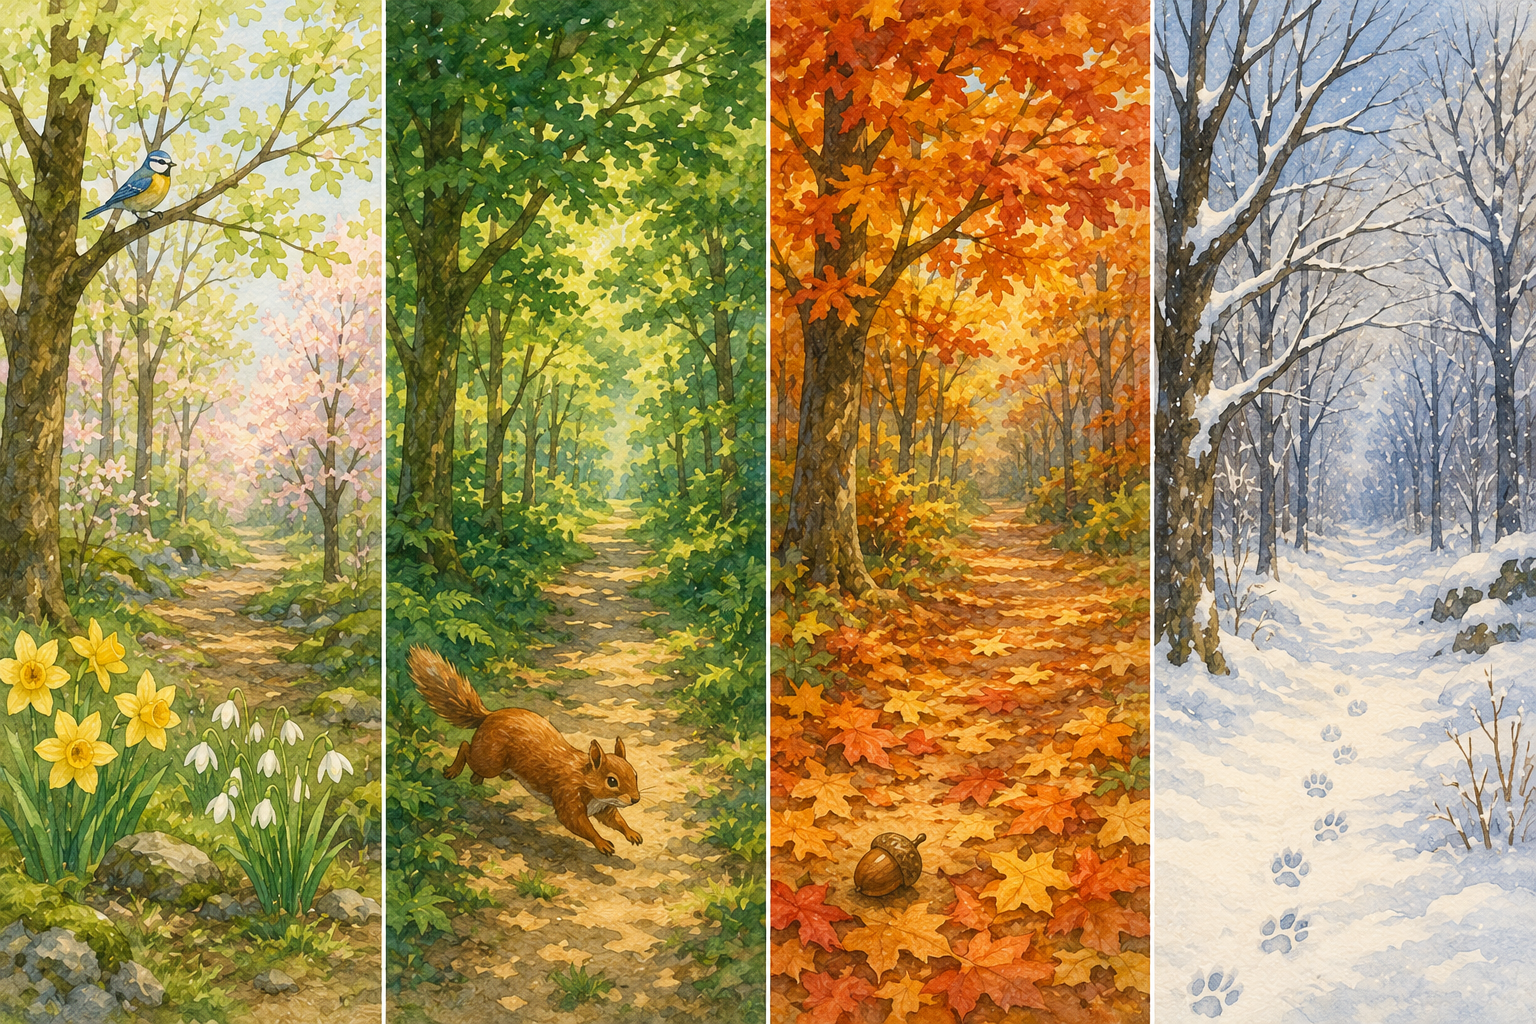
\includegraphics[width=7cm]{img/saisons.png}
\end{wrapfigure}

La forêt n'est jamais la même. Elle change tout au long de l'année.
Chaque saison apporte ses couleurs, ses odeurs et ses bruits.

\textbf{Le printemps : la forêt se réveille}

Au printemps, la forêt sort de son long sommeil d'hiver. Les arbres font
de petites feuilles toutes neuves, d'un vert très clair. Le sol se
couvre de fleurs : on voit des jonquilles jaunes, des violettes et des
perce-neige.

Les oiseaux reviennent et chantent dès le matin. Les écureuils sortent
de leurs cachettes. Sous la terre, les graines se réveillent et
commencent à pousser. C'est aussi la saison des bébés animaux : les
renardeaux et les jeunes chevreuils naissent au printemps.

\textbf{L'été : la forêt est verte}

En été, la forêt est très verte. Toutes les feuilles sont grandes et
épaisses. Elles font de l'ombre. Quand il fait très chaud dehors, il
fait plus frais sous les arbres. C'est très agréable de s'y promener.

Les animaux se cachent souvent pendant la journée. Ils sortent surtout
le matin tôt ou le soir, quand il fait moins chaud. Beaucoup de petits
fruits commencent à pousser : les noisettes, les mûres et les framboises
sauvages.

\textbf{L'automne : la forêt change de couleur}

L'automne, c'est ma saison préférée. Les feuilles passent du vert au
jaune, puis à l'orange et au rouge. La forêt ressemble à une grande
peinture pleine de couleurs.

Puis les feuilles tombent. Elles font un tapis épais sur le sol. Quand
on marche dessus, ça fait « crac crac ». Les arbres laissent tomber
leurs fruits : glands, châtaignes et noisettes. Les écureuils sont très
occupés. Ils font des réserves pour passer l'hiver.

Les champignons poussent partout, sous la pluie et dans la mousse. Mais
attention : il ne faut jamais ramasser un champignon tout seul. Certains
sont très dangereux.

\textbf{L'hiver : la forêt dort}

En hiver, la forêt est calme et silencieuse. Les arbres ont perdu toutes
leurs feuilles. Les branches sont nues et noires. Parfois, la neige les
recouvre. Tout est blanc et tout est beau.

Beaucoup d'animaux dorment pendant l'hiver. Les hérissons et les
marmottes hibernent. Ils ne se réveilleront qu'au printemps suivant.
D'autres animaux, comme les renards, restent éveillés. Mais ils ont du
mal à trouver à manger.

Si tu marches dans la forêt en hiver, tu peux voir des traces de pas
dans la neige. Ces empreintes te racontent tous les animaux qui sont
passés par là pendant la nuit.

La forêt est belle en toutes saisons. Il faut juste savoir l'observer.

\begin{center}\rule{0.5\linewidth}{0.5pt}\end{center}

\subsubsection{Questions de
compréhension}\label{questions-de-compruxe9hension-14}

\begin{enumerate}
\def\labelenumi{\arabic{enumi}.}
\tightlist
\item
  Quelle saison réveille la forêt ?
\item
  Pourquoi les écureuils sont-ils très occupés en automne ?
\item
  Que peut-on voir dans la neige en hiver, et qu'est-ce que cela nous
  raconte ?
\end{enumerate}

\begin{center}\rule{0.5\linewidth}{0.5pt}\end{center}

\subsubsection{Mon suivi de lecture}\label{mon-suivi-de-lecture-14}

\begin{center}
\begin{tabularx}{0.75\textwidth}{|X|X|}
\hline
\textbf{Date} & \textbf{Temps} \\
\hline
& \\
\hline
& \\
\hline
& \\
\hline
& \\
\hline
& \\
\hline
\end{tabularx}
\end{center}

\begin{center}\rule{0.5\linewidth}{0.5pt}\end{center}

\newpage

\section{Lettre du bout du monde}\label{lettre-du-bout-du-monde}

\begin{wrapfigure}{r}{7cm}
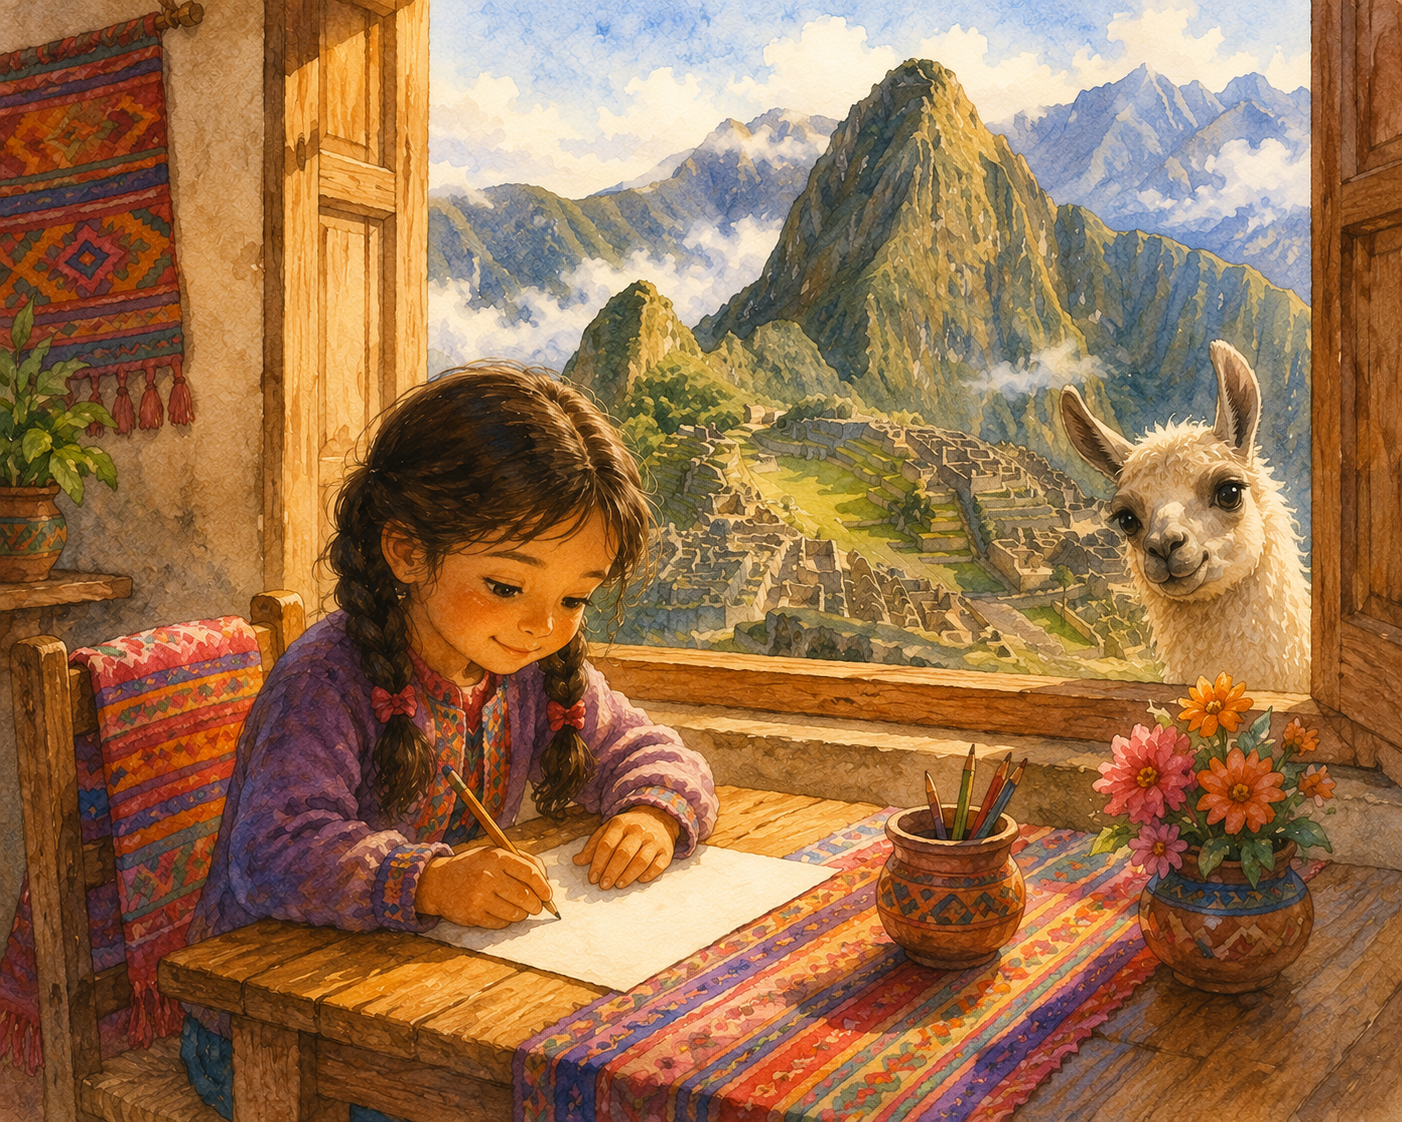
\includegraphics[width=7cm]{img/perou.png}
\end{wrapfigure}

Chère Mamie,

Je t'écris depuis le Pérou ! C'est un pays très loin de la France, en
Amérique du Sud. Cela fait déjà trois semaines que nous voyageons avec
papa, maman et mon petit frère. J'ai tant de choses à te raconter !

Au début, nous étions à Lima, la grande capitale. C'est une ville
bruyante, posée au bord de la mer. J'ai goûté du poisson cru avec du
citron. Ici, ils appellent ça du « ceviche ». C'était surprenant, mais
bon.

Ensuite, nous avons pris un avion pour aller à Cusco. Cusco est une
ville en haut dans les montagnes. Là-bas, l'air est très fin. Au début,
j'étais essoufflée juste en montant les escaliers ! Maman dit que c'est
à cause de l'altitude. Quand on est très haut, il y a moins d'air à
respirer.

Le plus beau, c'est quand nous sommes allés voir le Machu Picchu. Tu
connais peut-être ? C'est une vieille ville construite tout en pierres,
posée tout en haut d'une montagne. Elle a été bâtie il y a très, très
longtemps par les Incas. Les Incas étaient un peuple ancien d'Amérique.
Ils faisaient des choses incroyables sans machine, juste avec leurs
mains.

Pour monter au Machu Picchu, nous avons marché longtemps. C'était dur,
mais quand je suis arrivée tout en haut, j'avais oublié toute ma
fatigue. J'ai vu des nuages plus bas que moi ! Imagine : je regardais le
ciel par en dessous. Et autour, il y avait des montagnes vertes à perte
de vue. Je n'avais jamais rien vu d'aussi beau.

Au Pérou, j'ai aussi rencontré des animaux nouveaux pour moi. Les lamas
sont mes préférés. Ils ressemblent à de grands moutons avec un long cou.
Ils crachent quand on les énerve ! Heureusement, je suis restée polie
avec eux. J'ai aussi vu des perroquets aux mille couleurs et de très
grands oiseaux qui volent très haut, les condors.

Les gens ici sont très gentils. Ils sourient beaucoup. Beaucoup d'entre
eux parlent une langue spéciale, en plus de l'espagnol. Cette langue
s'appelle le quechua. J'ai appris à dire « bonjour » : « allillanchu ».
C'est joli, tu ne trouves pas ?

Demain, nous partons à la campagne. Nous allons dormir une nuit dans une
vraie maison péruvienne. J'ai un peu peur, parce que parfois il n'y a
pas d'eau chaude. Mais je crois que je vais quand même bien m'amuser.

Je pense à toi tous les jours. Je te raconterai tout en rentrant à la
maison. Je t'ai déjà acheté un petit cadeau. Mais c'est une surprise !

Je t'embrasse très fort,

Ta petite Camille.

\begin{center}\rule{0.5\linewidth}{0.5pt}\end{center}

\subsubsection{Questions de
compréhension}\label{questions-de-compruxe9hension-15}

\begin{enumerate}
\def\labelenumi{\arabic{enumi}.}
\tightlist
\item
  Dans quel pays se trouve Camille ?
\item
  Pourquoi était-elle essoufflée à Cusco ?
\item
  Que font les lamas quand on les énerve ?
\end{enumerate}

\begin{center}\rule{0.5\linewidth}{0.5pt}\end{center}

\subsubsection{Mon suivi de lecture}\label{mon-suivi-de-lecture-15}

\begin{center}
\begin{tabularx}{0.75\textwidth}{|X|X|}
\hline
\textbf{Date} & \textbf{Temps} \\
\hline
& \\
\hline
& \\
\hline
& \\
\hline
& \\
\hline
& \\
\hline
\end{tabularx}
\end{center}

\begin{center}\rule{0.5\linewidth}{0.5pt}\end{center}

\newpage

\section{Bilan général}\label{bilan-guxe9nuxe9ral}

Note ici tes records personnels !

\subsubsection{Section 1 --- Textes
courts}\label{section-1-textes-courts-1}

{\def\LTcaptype{none} % do not increment counter
\begin{longtable}[]{@{}llll@{}}
\toprule\noalign{}
Texte & Mon meilleur temps & Mots / minute & Date \\
\midrule\noalign{}
\endhead
\bottomrule\noalign{}
\endlastfoot
Les animaux de la mer & & & \\
Je fais du vélo & & & \\
Ma copine Sara & & & \\
Ma cabane secrète & & & \\
\end{longtable}
}

\subsubsection{Section 2 --- Niveau 1}\label{section-2-niveau-1-1}

{\def\LTcaptype{none} % do not increment counter
\begin{longtable}[]{@{}llll@{}}
\toprule\noalign{}
Texte & Mon meilleur temps & Mots / minute & Date \\
\midrule\noalign{}
\endhead
\bottomrule\noalign{}
\endlastfoot
Mon chat Filou & & & \\
Je plante des radis & & & \\
Le premier jour de Mango & & & \\
À la patinoire & & & \\
\end{longtable}
}

\subsubsection{Section 3 --- Niveau 2}\label{section-3-niveau-2-1}

{\def\LTcaptype{none} % do not increment counter
\begin{longtable}[]{@{}llll@{}}
\toprule\noalign{}
Texte & Mon meilleur temps & Mots / minute & Date \\
\midrule\noalign{}
\endhead
\bottomrule\noalign{}
\endlastfoot
Les habitants de la forêt & & & \\
Une journée à Tokyo & & & \\
Comment poussent les plantes & & & \\
Le chat des voisins & & & \\
\end{longtable}
}

\subsubsection{Section 4 --- Niveau 3}\label{section-4-niveau-3-1}

{\def\LTcaptype{none} % do not increment counter
\begin{longtable}[]{@{}llll@{}}
\toprule\noalign{}
Texte & Mon meilleur temps & Mots / minute & Date \\
\midrule\noalign{}
\endhead
\bottomrule\noalign{}
\endlastfoot
Le spectacle sur glace & & & \\
Médor, le chien qui voit pour Léon & & & \\
Les quatre saisons de la forêt & & & \\
Lettre du bout du monde & & & \\
\end{longtable}
}

\textbf{Objectif} : lire de plus en plus vite, et toujours en comprenant
ce qu'on lit. Bravo pour tes efforts !

\newpage

\vspace*{2cm}
\begin{center}
{\fontsize{38pt}{44pt}\selectfont\bfseries À propos de ce livret}\\[1em]
\textcolor{accentcolor}{\rule{0.35\textwidth}{1.5pt}}
\end{center}
\vspace{1.5cm}

\subsubsection*{Pourquoi ce livret existe}

Ce livret a été créé pour ma fille, qui avait du mal à lire à la vitesse attendue à son âge. Il est offert \textbf{gratuitement} à toutes les familles, enseignant·e·s et orthophonistes qui pensent qu'il peut être utile.

\subsubsection*{Partage et licence}

\textbf{Tu peux librement :}
\begin{itemize}
\tightlist
\item le télécharger, l'imprimer et le distribuer,
\item le modifier, l'adapter, le traduire (par exemple pour un autre prénom),
\item le partager avec d'autres parents, enseignants, orthophonistes ou amis.
\end{itemize}

\textbf{À condition de :}
\begin{itemize}
\tightlist
\item ne pas l'utiliser à des fins commerciales (pas de vente),
\item garder la même licence libre pour tes adaptations,
\item mentionner l'auteur·e original·e.
\end{itemize}

\vspace{0.5em}

\textbf{Licence :} Creative Commons Attribution – Pas d'Utilisation Commerciale – Partage dans les Mêmes Conditions 4.0 International (\textbf{CC BY-NC-SA 4.0}).

{\small Texte complet : \url{https://creativecommons.org/licenses/by-nc-sa/4.0/deed.fr}}

\subsubsection*{Donner ton avis}

Si ce livret a aidé un enfant, j'aimerais beaucoup le savoir.

\begin{center}
\textbf{\url{https://TON-LIEN-LANDING-PAGE.example.com}}
\end{center}

\vfill

\begin{center}
\textit{Si ce livret t'a aidé·e, le plus beau remerciement, c'est de le partager à une autre famille qui en aurait besoin.}
\end{center}

\vspace{1cm}

\end{document} 